\documentclass[preprint,12pt,authoryear]{elsarticle}

\IfFileExists{mmap.sty}{\usepackage[noTeX]{mmap}}{}
%\usepackage{fancyhdr}
\usepackage{amsfonts}
%\usepackage{epsfig}
\usepackage{amsmath}
%% The amssymb package provides various useful mathematical symbols
\usepackage{amssymb}
%% The amsthm package provides extended theorem environments
\usepackage{amsthm}
\usepackage{bbm}%% step function or indicate function
\usepackage{color}
% \usepackage{xcolor}
% \usepackage[dvipsnames]{xcolor}
\usepackage{setspace}
\usepackage{ragged2e}

%\newtheorem{remark}{Remark}
%\newtheorem{theorem}{Theorem}[section]
\newtheorem{theorem}{Theorem}
\newtheorem{assumption}{Assumption}
%\newtheorem{lemma}[theorem]{Lemma}
% \numberwithin{equation}{section}
%\newtheorem{definition}[theorem]{Definition}
\newtheorem{example}{Example}

\usepackage{subfigure}
%\usepackage{subcaption}
\usepackage{graphicx}
\usepackage{paralist}
\usepackage{longtable}

\usepackage{multirow}
%\definecolor{darkblue}{rgb}{0.0,0.0,0.3}
% \usepackage{hyperref}
% \hypersetup{colorlinks,breaklinks, linkcolor=darkblue,urlcolor=darkblue, anchorcolor=darkblue,citecolor=darkblue,bookmarksopen=true}
\usepackage{ulem}
\usepackage{ifthen}
\usepackage{booktabs}
\usepackage{threeparttable}
\usepackage[figureright]{rotating}
\usepackage{epsfig}
\usepackage{epstopdf}
% \usepackage[colorlinks,linkcolor=red,anchorcolor=blue,citecolor=green,CJKbookmarks=True]{hyperref}
\usepackage{hyperref}
\hypersetup{
  pdftitle={An awesome paper},
  pdfauthor={Zijin Wang, Peimin Chen}
}
%\usepackage{blindtext}

\let\originalepsffile\epsffile
\renewcommand{\epsffile}[1]{\originalepsffile{Peimin/#1}}
\renewcommand{\thefigure}{\arabic{figure}}
%\renewcommand{\thesubfigure}{\thefigure{}\alph{subfigure}:}
\renewcommand{\thesubfigure}{Panel \Alph{subfigure}.}
%\renewcommand {\thefigure} {\thechapter{}.\arabic{figure}}
 %\@thesubfigure
%\newcommand{\reffig}[1]{Figure \ref{#1}}

\vfuzz2pt % Don't report over-full v-boxes if over-edge is small
\hfuzz2pt % Don't report over-full h-boxes if over-edge is small

\addtolength{\topmargin}{-0.6in}
\addtolength{\topskip}{0.0in}    % between header and text
\addtolength{\textheight}{1.5in} % height of main text
\addtolength{\textwidth}{0.8in}    % width of text
\addtolength{\oddsidemargin}{-0.4in} % odd page left margin
\addtolength{\evensidemargin}{-0.4in} % even page left margin

\newcommand{\documentspacing}{\linespread{1.4}}
\newcommand{\condensedspacing}{\linespread{1.1}}  % 1.5
\documentspacing
\newcommand{\Anonymize}{NO} % Do not anonymize
\vspace{30 mm}


\begin{document}
% \begin{sloppypar}

% \phantomsection
\begin{frontmatter}

\title{ Volatility Forecasts by Clustering: Applications for VaR Estimation } %\tnoteref{label0}}

\vskip 1.5cm

\author{ {\large Zijin Wang}\\ School of Economic Mathematics \\
Southwestern University of Finance and Economics\\ Chengdu,
611130, P.R. China \\
 Tel: +86-15884554480\\ E-mail: 1190202Z1006@smail.swufe.edu.cn \vskip 0.5cm
{\large Peimin Chen{\small*}}\\School of Hospitality Management\\Shanghai Business School \\
Shanghai, 200235, P.R. China \\
 Tel: +86-18328516475\\ E-mail: pmchen@sbs.edu.cn  \vskip 0.5cm
{\large Peng Liu }\\S.C. Johnson College of Business\\Cornell University\\
Ithaca, NY, 14853, USA\\
Tel: 510-277-2874\\ Fax: 607-254-2960\\  E-mail:
peng.liu@cornell.edu
 \vskip 0.5cm and  \vskip 0.5cm
{\large Chunchi Wu{\small*}} \\ School of Management\\
  State University of New York\\
  Buffalo, NY, 14260, USA\\
  Tel: 716-645-0448\\ Fax: 716-645-3823\\
  E-mail: chunchiw@buffalo.edu
%\vskip 1cm Current version: June 5, 2021.
\newpage
\begin{center}
{\Large Volatility Forecasts by Clustering: Applications for VaR Estimation }
\end{center}
  }
\cortext[cor2]{Corresponding author.}
\begin{abstract}
It is well known that volatility is time-varying and clustered. However, few studies have explored the information content of volatility clustering and its implications for investors' risk aversion.  This information is particularly important in turbulent periods, such as financial crisis. We present a volatility cluster partition model to forecast volatility and apply it to risk management. We find that our model substantially outperforms the GARCH model and improves financial risk management using the value-at-risk metric.
\end{abstract}

\begin{keyword}
Volatility forecasts; Fisher's optimal dissection;
value-at-risk. %option pricing; GARCH-MIDAS model.
\end{keyword}

%{\it JEL classification:} G35; G01

\end{frontmatter}

% \mainmatter
\section{Introduction} % unrevised
\label{sec:Introduction} Return volatility is an important risk factor in asset pricing, portfolio selection and risk management (see \cite{Angelini2019}; \cite{Schmitt2017}; \cite{Engle2018}; \cite{Chen2019}). To capture instantaneous volatility dynamics and clustering, the classic Autoregressive Conditional Heteroskedasticity (ARCH) model and Generalized Autoregressive Conditional Heteroskedasticity (GARCH) model proposed  by \cite{Engle1982} and \cite{Bollerslev1986} are popular for its simplicity and ease to interpret. Extended work, such as \cite{Nelson1991} and \cite{Engle1993}), examine the properties of asymmetry and high persistence.
However, the GARCH-type models have some weaknesses. These models often 
have poor performance in describing rapid volatility changes in financial markets (see \cite{Andersen2003}, \cite{Hansen2012} and \cite{Smetanina2021}) and produce poor forecasts.
On the other hand,
for most financial models involving dynamic volatility (such as Heston model, CEV model, etc.), it is hard to estimate their parameters jointly using the real data, because many factors are involved and the likelihood functions are not easy to derive.
For application purposes, it is desirable to have a simple volatility measure, which can incorporate current market information promptly. In this paper, we propose a volatility cluster partition model based on the clustering analysis to forecast return volatility. This model captures market information in real time and is easy to implement. Applying our model to risk management using the value-at-risk (VaR) metric, we find that it outperforms conventional methods by a substantial margin.

%Earlier studies on return volatility use the historical data measure
%(see \cite{Fama1965}). %Historical volatility assumes that the
%%future is an extension of the past, so historical data can be used
%%to estimate volatility.
%The historical measure is simple but inaccurate as it uses
%past volatility as a proxy for future
%volatility. As such, it has limited uses in practice.
%Classical financial theory assumes that asset returns follow
%an independent identical normal distribution, and
%adopts standard deviation as the risk of a financial asset (see
%\cite{Mandelbrot1967}). However, it is well known that returns are not independently distributed and
%volatility is a time-dependent random variable, which can be
%described by a time-series model (see \cite{Engle1982}), such as the generalized
%autoregressive conditional heteroskedasticity (GARCH) model (see
%\cite{Bollerslev1986};

Stock prices can change abruptly and it is important to accommodate such a feature in volatility forecasts. As an example, since its introduction, the circuit breaker has been triggered only once on October 27, 1997, when the Dow Jones industrial index fell 7.18\%, before 2020. However, from March 9 to March 18, 2020, the circuit breaker was triggered four times. Particularly, on March 16, the S\&P 500 index triggered a circuit breaker at the market open for the first time in history, and the index experienced the largest one-day decline in nearly 33 years with a drop of 11.98\%. Over this period, market volatility was extremely high. Ignoring the structure shift in time series can lead to inefficient volatility forecasts.

Volatility exhibits pronounced clustering. It can remain stable over a period of time but
suddenly switch to another state.
When volatility is in a stable mode, dynamic variations are a lesser concern and the mean of volatility is the main focus of attention.
Thus, we can use the average value of volatility during a stable
	period as a representative volatility measure to determine the optimal time points for cluster partitions.
\cite{Schmitt2017} put forward that the herding behaviour of speculators
	leads to volatility clustering. When the market is calm, investors make decisions
	independently. But during the turbulent period, market participants are sensitive to other people's behaviour and they concentrate either on the buy or sell side. Under the unbalanced trading condition, stock prices adjust dramatically and volatility remains high.
	
	The calm or turbulent state is usually quite persistent. However, external shocks	such as financial crisis, wars 
	or drastic changes in government policies can quickly change the regime.
	This can be characterized by a regime-switching (RS) process.  For the RS models, a Markov process with
	state-dependent transition probabilities governs the switching between regimes. The maximum
	likelihood method is employed for the statistical inference on the optimal regime.
	\cite{Hamilton1989} introduces this model to describe the U.S. business cycle, which is characterized
	by periodic shifts from recessions to expansions and vice versa. \cite{Klaassen2002} proposes
	RS-GARCH models, in which GARCH is used in each regime to describe the volatility process.
	\cite{Pelletier2006} proposes an alternative volatility model for multiple time series with the regime switching
	dynamic correlation. The covariance is a constant within a regime but changes across regimes.
	
	Signals of RS models can be phrased as structural change points, which has been traditionally detected
	by hypothesis tests (see, for example, \cite{Andreou2002} and \cite{Lee2015}).
	\cite{Brown1974}
	modify the Levene test on the equality of ex-ante and ex-post variance changes and this test is widely
	used in studies of stock prices (see \cite{Riordan2012}) and futures markets (see \cite{Ederington1993}).
	
	Clustering analysis such as $k$-mean, mean-shift clustering algorithm (see \cite{Cheng1995}), and density-based spatial clustering with noise (DBSCAN, see \cite{Ester1996}), has gained popularity in past two decades and has been developed and extended in many applied fields from statistics (see \cite{Jain1999}) to image segmentation (see \cite{Coleman1979}). More complicated methods, including support-vector machine and neural networks, are developed in artificial intelligence (see, for example, \cite{Zhang2000};  \cite{Shi2016}). It has been shown that these methods are efficient in dealing with the data without time order. However, in most financial models, the data involved follows a time series process and it is therefore necessary to find an alternative method to cluster the series. The Fisher's optimal dissection method is a suitable algorithm for financial modeling as it can cluster dynamic volatility by minimizing a loss function defined by the similarity of samples. The basic idea of this method is widely employed in economics (see \cite{Bai2003}) and image treatment (see \cite{Verbesselt2010}).
	
	In this paper, we use Fisher's optimal dissection method to model return volatility. Using this method, we identify the time points for volatility clustering and use the representative value of volatility for a stable period. For a new updated data, we can easily examine whether it belongs to the latest cluster or not. If it is, then the representative value of this cluster can be employed to predict the future volatility. If not, it is a signal of regime switch, and we need to cluster the series differently in order to produce a better volatility forecast.

%Conventional methods in cluster analysis, such as $k$-mean
%algorithm (see \cite{MacQueen1967}), mean-shift clustering algorithm (see \cite{Cheng1995}), and density-based spatial
%clustering with noise (DBSCAN, see \cite{Ester1996}), have been
%developed and extended in many applied fields from statistics (see \cite{Jain1999}) to image segmentation (see \cite{Coleman1979}). More complicated methods with parameters, including support-vector machine and neural networks, are developed in artificial intelligence (see, for example, \cite{Zhang2000};  \cite{Shi2016}). It has been shown that these
%methods are efficient in processing the data with no time
%order. However, in most financial models, the data involved
%follows a time series process and it is therefore necessary to find
%an alternative method to cluster the series. The Fisher
%optimal dissection method is a suitable algorithm for
%financial modeling as it can cluster dynamic volatility by
%minimizing a loss function defined by the similarity of samples. The basic idea of such a method is widely employed in economics (see \cite{Bai2003}) and image treatment (see \cite{Verbesselt2010}).

Our model differs from the conventional models for structural changes in two major aspects.
First, our model performs optimal volatility partitions and generates timely classification by
incorporating the most updated market information.
To identify the optimal classification, few observations
are sufficient to implement our method.
Thus, our model can capture market information much faster. This procedure
contrasts with the tests commonly used in prior research that relies on the statistical inference on the
parameters of the model. In these tests, the occurrence of the structural change in parameters only reveals
after enough samples are produced. As such, it cannot capture instantaneous fluctuations in volatility.
To catch market information flows immediately, a more efficient method is needed. Second, the algorithm
we develop is convenient and general, and there is no need to derive the inference for test statistics.
It is not easy to draw an efficient statistical inference for the structural change or regime-switching
model of the implied volatility calculated from the option pricing formula by the iteration method.
An advantage of our algorithm is that it can incorporate the newly calculated implied volatility into the model 
to quickly infer the structural change.

%Mathematical finance scholars proposed the concept of stochastic
%volatility. They established stochastic processes with random
%fluctuations of volatility over time, including discrete and
%continuous forms of stochastic models (see Poterba \& Summers
%1984). In these models, the noise term of the added volatility
%makes the model more flexible, but analytical solutions are hardly
%available. Thus, it is difficult to estimate the parameters of
%these models.

%With the development of computer technology and the internet
%technology, interdisciplinary research has gradually emerged (see
%Chuong \& Nikolai, 2018). Applying computer technology to the
%financial field to solve some complex calculations has contributed
%to some complicated models. In the past, some complicated models
%without analytical solution, can only be numerically calculated by
%means of computer programs after computer technology, which
%greatly improves the computational efficiency and the application
%range of the model.

%Estimation of volatility has been a difficult problem in the financial field.
%This paper aims to find a way to periodically describe the volatility of a
%certain period of time, which can replace the method of constant volatility
%and the method of real-time estimation of volatility at any time point.


%Value-at-risk (VaR) is a standard indicator for market risk used
%by financial institutions and banking regulators. A VaR estimation
%corresponds to a specific critical value of potential loss
%probability distribution for a porifolio or an asset (see Kupic
%1995). Different methods have been used to calculate VaR value
%(e.g. Jorion 1996; P$\mathrm{\acute{e}}$rignon and Smith 2008;
%Orhan and K$\mathrm{\ddot{o}}$ksal 2012; Godeiro 2014).

%This paper uses the data mining algorithm in the computer to make
%appropriate improvements to the volatility model, and then applies
%it to the calculation of market risk VaR.

The GARCH model has been widely used for volatility forecasts by academicians and practitioners. \cite{Orhan2012}
compare various GARCH models for quantifying the VaR in times of stress.
VaR measures the maximum likely loss of an investment portfolio
within a certain time period at a confidence level.
There are several main methods to estimate VaR, such as nonparametric histotical simulation and parametric variance-covariance models.
In this paper, we choose GARCH as a benchmark to evaluate the
performance of our model in VaR applications. We also consider other volatility models such as RSGARCH, HAR and asymmetric HAR and evaluae their performance.

This paper makes several contributions to the current literature. First, we propose a new model
to cluster dynamic volatility using Fisher's
optimal dissection method. A unique feature of our model is that the simulated
volatility is a constant in each cluster section but can
promptly respond to shocks at the cluster partition point.
Second, unlike previous models, estimating the parameters of our model is relatively straightforward and the model is easy to implement. Third, our model outperforms the traditional GARCH model in volatility forecasts.
Using the volatility simulated by our model, we find that it significantly improves the performance of risk management using
the VaR metric. %and the prediction of option prices.
The clustering volatility estimated by our model
tracks real volatility much more closely than the standard GARCH model and delivers superior forecasts for future volatilities.
%In addition, using our method improves the estimation and forecasts of the GARCH-MIDAS model.

%the basic trend of volatility is predicted by GARCH model, which
%reflects the characteristics of volatility, such as volatility
%clustering. Secondly, due to the inconvenience of GARCH model,
%clustering analysis technology is introduced and a structural
%change model of volatility is proposed. Finally, the structural
%model of volatility is applied to the VaR calculation and the
%empirical analysis is carried out.

The remainder of this paper is organized as follows. In Section 2,
we introduce the different dynamic models of volatility.
In Section 3, we present the cluster model based on
Fisher's optimal dissection method. In Section 4, we discuss the
applications of our volatility measures to VaR and option price predictions
and show that our method enhances the forecast of the HAR model.
In Sections 5, we provide empirical results of volatility forecast and VaR.
Finally, in Section 6, we summarize our main findings and conclude the paper.


\section{Volatility cluster model}
In this section, we provide a concise review of the classical GARCH model and recent volatility models and compare their structures.

\subsection{GARCH volatility model}
Assume that the time series of returns $r_t$, $t=1,\dots,T$ has the following process:
\begin{align}\label{equa1}
	r_t&=\mu_t+ e_t, \notag\\
	e_t&=\sigma_t\varepsilon_t,  \notag\\
	\varepsilon_t&\sim D(0,1),
\end{align}
where $\mu_t$ is the dynamic mean and $e_t$ is residual, $\{\varepsilon_t\}$ is an independent and identically distributed innovation process with mean zero and unit variance and $\sigma_t>0$ is the conditional volatility independent of $\{\varepsilon_t\}$. The conditional variance is measured on the past information $\mathcal{F}_{t-1}$, $\sigma_t^2=\mathbb{E}[r_t^2|\mathcal{F}_{t-1}].$

In the presence of volatility clustering, it is clear that $\sigma_t$ is not independent but correlated to both time and previous states. The most important models measuring volatility clustering are Autoregressive Conditional Heterogeneous (ARCH) and the extended General Autoregressive Conditional Heterogeneous (GARCH) model proposed by \cite{Engle1982} and \cite{Bollerslev1986}, respectively. A typical GARCH(p,q) can be written as
\begin{equation}
	\sigma_t^2=\omega+\sum_{i=1}^q\alpha_i r_{t-i}^2+ \sum_{j=1}^p\beta_j \sigma_{t-j}^2,
\end{equation}
where $\omega$ is parameter, $\alpha_i$ are ARCH parameter and $\beta_j$ are GARCH parameter.
The conditonal variance is typically parametrized with $p=1$ and $q=1$ as
\begin{equation}
	\sigma_t^2=\omega+\alpha r_{t-1}^2+\beta \sigma_{t-1}^2.
\end{equation}

The standard GARCH is a convenient model that can generate a stationary process. However, it has some weaknesses. For example, it cannot model volatility asymmetry widely documented in the literature. In reality, bad news have a larger impact on volatility than good news (\cite{Conrad2020}), but the standard GARCH cannot not differentiate these effects.
There are more elaborated recursive structures that can imposed to improve the standard GARCH model (see \cite{Glosten1993}). For the GJR-GARCH model, the conditional volatility is formulated as
\begin{equation}
	\sigma_t^2=\omega+\alpha r_{t-1}^2 +\gamma r_{t-1}^2\mathbbm{1}_{r_{t-1}<0} +\beta \sigma_{t-1}^2,
\end{equation}
where $\mathbbm{1}_{r_{t-1}<0}$ is an indicator function and $\gamma$ is leverage parameter.

% The Exponential GARCH (EGARCH) is proposed by \cite{Nelson1991}, the conditional variance in EGARCH(1,1) is a multiplicative function of lagged innovations,
% \begin{equation}
% 	\log\sigma_t^2=\omega+\alpha\left(|\varepsilon_{t-1}|-\mathbb{E}|\varepsilon_{t-1}|\right)+\beta\log\sigma_{t-1}^2+\gamma \varepsilon_{t-1},
% \end{equation}
% where $\gamma$ is the asymmetric parameter. Positive and negative have different effect on conditional variance.


A weakness of the GARCH models is that they can not include latest volatility timely.
For example, when a new return data arrives which is a drastic decrease or increase, the model will just take it into estimation with the whole data sample. This new data cannot change the parameter estimate significantly and the model cannot detect whether it is an outlier of innovation or a change of volatility.

The GARCH-type models are poorly equipped for capturing rapid changes in financial markets as pointed out by \cite{Andersen2003}, \cite{Hansen2012} and \cite{Smetanina2021}, and thus give poor volatility forecasts. Especially in rapid changing periods, the forecasts are more inaccurate compared to the calm period.

\subsection{Regime switching GARCH}

Volatile and calm periods typically represent different regimes. Markov Regime Switch models are well suited to model different regimes.
In these models, returns are dependent on state
\begin{equation}
	r_t=\sigma_{s_t}\varepsilon_t,
\end{equation}
where $s_t\in \{1,\dots,N\}$ is a random variable of state at date $t$, satisfying a Markov process
\begin{equation}
	P(s_t=j|s_{t-1}=i,s_{t-2},\cdots,r_{t-1},r_{t-2},\cdots)=P(s_t=j|s_{t-1}=i)=p_{ij},
\end{equation}
where $p_{ij}$ is the probability of switching from state $i$ to $j$ with $i,j\in 1,\cdots,N$.

\cite{Haas2004} proposes a regime switching GARCH (RSGARCH) model where there are $N$ separate GARCH processes whose conditional volatility $\sigma_{it}$ all exist as latent variables at time $t$,
\begin{equation}
	\sigma_{it}^2=\omega_i+\alpha_i r_{t-1}^2+\beta_i \sigma_{i,t-1}^2,
\end{equation}
where parameters $\omega_i, \alpha_i$ and $\beta_i$ are dependent on state $i\in \{1,\dots,N\}$.\footnote{For estimation, we use a MATLAB toolbox \textit{RSGARCH} provided in \cite{Chuffart2017}.}

In practice, most applications assume only $N=2$ or $3$ different regimes though there are other models accommodating a larger number of regimes either by tightly parameterizing the relation between regimes (see \cite{Calvet2004}) or with prior Baysian information as \cite{Sims2006}. Estimation gets complicated with more regimes, and for simplicity and without loss of generality, we focus on the case of two regimes in the performance evaluation of different models.

\subsection{HAR-RV}

Realized variance (RV) is an empirical measure of daily return variability, constructed from cumulative squared intraday returns
\begin{equation*}
	RV_t^M=\sum_{i=1}^{M}r_{t,i}^2,
\end{equation*}
where $r_{t,i}$ is the $i$th logarithmic return during day $t$, $M$ is the number of returns in each day. As $M$ increases to infinity, RV is a consistent estimate of true variance (see \cite{Andersen1998}, \cite{Barndorff-Nielson2002}, \cite{Andreou2009}).

Market microstructure dynamics contaminate the price process with noise, which can be time dependent and may be correlated with the efficient price (Hansen and Lunde, 2006). RV can be a biased and inconsistent estimator.\footnote{For more details on the effects of market microstructure noise on volatility estimation, please refer to Bandi and Russell (2006), Hansen and Lunde (2006), Oomen (2005), and Zhang et al. (2005).} To reduce the effect of market microstructure noise, \cite{Liu2008} employ a kernel-based estimator that utilizes autocovariances of intraday returns. Specifically, \cite{Liu2008} follow Hansen and Lunde (2006) to provide a bias correction to realized volatility as
\begin{equation*}
	RV_t^M=\sum_{i=1}^{M}r_{t,i}^2+2\sum_{h=1}^{q}(1-\frac{h}{q+1})\sum_{i=1}^{M-h}r_{t,i}r_{t,i+h},
\end{equation*}
where $q=1$ in this calculation.

\cite{Corsi2008} considers the heterogeneous autoregressive model (HAR) of realized volatility, which can capture many features of volatility including long memory.
The logrithmic of the HAR is defined as:
\begin{equation}\label{HAR}
	v_t=b_0+b_1v_{t-1}+b_2v_{t-5,t-1}+b_3v_{t-22,t-1}+\varepsilon_t,
\end{equation}
where $\varepsilon_t\sim D(0,\sigma^2)$, $v_t=\log(RV_t)$ and
\begin{equation*}
	v_{t-5,t-1}=\frac{\log(RV_{t-1})+\log(RV_{t-2})+\cdots+\log(RV_{t-5})}{5},
\end{equation*}
\begin{equation*}
	v_{t-22,t-1}=\frac{\log(RV_{t-1})+\log(RV_{t-2})+\cdots+\log(RV_{t-22})}{22}.
\end{equation*}
This model postulates three factors that affect volatility: daily log-volatility $v_{t-1}$, weekly moving average $v_{t-5,t-1}$, and monthly $v_{t-22,t-1}.$

To account for asymmetry and jumps, volatility can be modeled as
\begin{align}\label{HAR_Liu}
	v_t=&b_0+b_1v_{t-1}+b_2v_{t-5,t-1}+b_3v_{t-22,t-1}+b_JJ_{t-1}+a_{1}\frac{|r_{t-1}|}{\sqrt{RV_{t-1}}}\notag\\
	&+a_{2}\frac{|r_{t-1}|}{\sqrt{RV_{t-1}}}\mathbbm{1}_{r_{t-1}<0} +\epsilon_t,
\end{align}
where $J_{t-1}$ is a jump component defined as that in \cite{Liu2008}
\begin{equation*}
	J_t=\left\{
	\begin{matrix}
		\log(RV_t-RBP_t+1) & if \, RV_t-RBP_t>0 \\
		0 & otherwise \\
	\end{matrix}
	\right.
\end{equation*}
here $RBP_t=\frac\pi2\sum_{i=1}^{M-1}|r_{t,i}||r_{t,i+1}|$ is realized bi-power variation.

Later, we compare both original HAR model and asymmetry HAR of (\ref{HAR}) and (\ref{HAR_Liu}).

\section{Cluster partition}

When there is a volatility structural change, a period of high volatility is distinguished from a period of low volatility. A key feature in our model is to use the latest structural volatility to forecast future volatility. An important task then is to detect the point of the structure change in volatility.

Given a sequence of volatility $V=(\sigma_1,\dots,\sigma_T)$, let $I$ be a partition point, and $V$ is divided into two clusters if we have
\footnote{In fact, we can construct a statistic inference by Chi-square test for the series $\{v_i\}_{i=1}^T$ to search its partition point for two clusters. But here we adopt the simple form as the inequality (\ref{douguai1}) to be consistent with the latter Fisher's optimal dissection method.}
\begin{equation}\label{douguai1}
\sum_{i=1}^{T}( \sigma_i-\bar{\sigma}_i )^2 > \sum_{{i_1}=1}^{I-1}( \sigma_{i_1}-\bar{\sigma}_{i_1} )^2 + \sum_{{i_2}=I}^{T}( \sigma_{i_2}-\bar{\sigma}_{i_2} )^2, \end{equation}
where $\bar{\sigma}_i$, $\bar{\sigma}_{i_1}$ and $\bar{\sigma}_{i_2}$ are
the corresponding gathering centers of $\{\sigma_i\}_{i=1}^T$, $\{\sigma_{i_1}\}_{i_1=1}^{I-1}$ and $\{\sigma_{i_2}\}_{i_2=I}^{T}$, respectively, $I=2,\cdots,T$.
Generally, the arithmetic or geometric mean values of the corresponding samples including the given element are used.
To have an algorithm of fast speed and a simple form of model, we employ arithmetic mean values as gathering centers.
The greater the difference between the left side and
the right side, the more likely two different clusters.
As the sum of the left side of (\ref{douguai1}) is fixed, it is equivalent to minimizing the right side.
We construct the cluster statistic for a single structural change as
\begin{equation}\label{douguai2}
\rho_\sigma(I) =
\frac 1T\sum_{{i_1}=1}^{I-1}( \sigma_{i_1}-\bar{\sigma}_{i_1} )^2 +
\frac 1T\sum_{{i_2}=I}^{T}( \sigma_{i_2}-\bar{\sigma}_{i_2} )^2.
\end{equation}
The optimal partition point can be identified as ${\arg\min_{1\le i\le T}\rho_\sigma(i)}$ with the minimal sum of deviation, such that the volatilities in each cluster are alike and distinctly different across clusters.
This single break statistic is similar to the cumulative sum (CUSUM) test of a squared series (see \cite{Andreou2002} and \cite{Xu2013}). The difference between (\ref{douguai2}) and CUSUM is that we use conditional volatility instead. Although the squared return series is an unbiased estimator for variance, it usually contains noise.
Moreover, there may be more than one partition point. We can still use basic idea of minimizing the sum of deviation among clusters to construct a statistic for multiple structural changes.

% If we know the exact change point of volatility, we can do a test by F-statistic as \cite{Chow1960}. In practical,  we do not know when the volatility changes or even how many change point(s). One of the most widely used tests for volatility structural change is based on the cumulative sum (CUSUM) of squared series, see \cite{Andreou2002} and \cite{Xu2013}.


% GARCH family models usually contains infinite order information about conditional variances and errors, which may be irrelavant and even disturbing, especially when volatility changes dramatically.

% For example, by the sudden epidemic impact, the dramatic fluctuation of U.S. stock market volatility in March 2020 and 4 circuit breakers left investors with huge losses.
% If GARCH family models are used to forecast volatility, it will be underestimated due to the ineffectiveness of previous information.
% If forecast is based only on more recent data, precision will improve.
% Our model is to consider this point, through clustering we can find the most relevant time interval with the current time, and then use its representative cluster value to predict the volatility in short future.
%As GARCH family considers conditional variance as a lag model that contains information of very remote time which may cause problem especially in period when volatility change dramatically.

% $V=(\sigma^2_1,\dots,\sigma^2_T)$ are conditional variance and can be divided into $N$ clusters $C_1,\dots,C_N$. The representative value $\bar{\sigma}_N$ of the last cluster can be used as forecast $\sigma_{T+1}.$ This forecast has good properties of both original model and cluster partition model.

% \subsection{The statistic of determining single structural change point }\label{subsec:ClusterStatistic}

% In time series, it is important for researchers and
% financial analysts to discern a sequence transferring from one cluster to another as time goes by.
% This concern leads to two problems, known and unknown structural breaks.
% Traditional structural break problems have been phrased as hypothesis tests.
% The null is set up to describe structural stability, the alternative contains one or multiple structural break(s).
% Classical Chow Test (see \cite{Chow1960}) constructed $F$ statistic by linear regression before and after a structural break.
% Another popular way is to introduce dummy variable, and test all dummy variables and the interaction coefficient between dummy variables and independent variables.

% For unknown structural breaks, select a sub-interval and test every point in the sub-interval to derive the corresponding $F$ statistic.
% Take the largest $F$ statistic of them and then select the corresponding point as structural break.
% This $F$ statistic is also known as Quandt Likelihood Ratio (QLR).

% In general, the test statistics may be viewed as two-sample tests adjusted for the unknown break location.
% Often asymptotic relationships are derived to obtain critical values, see \cite{Bai1998}.

% To identify this pattern, we construct a statistic for cluster
% partitions. A partition point is
% selected with the minimum information loss, such that individual observations within the
% same cluster are alike while the difference between clusters is
% apparent.

% Let $I$ be a partition point, divide original data into two
% clusters if we have\footnote{In fact, we can construct a statistic inference by Chi-square test for the series $\{v_i\}_{i=1}^n$ to search its partition point for two clusters. But here we
% adopt the simple form as the inequality (\ref{douguai1}) to be consistent with the latter Fisher's optimal dissection method.}
% \begin{equation}\label{douguai1}
% \sum_{i=1}^{n}( \sigma_i-\bar{\sigma}_i )^2 > \sum_{{i_1}=1}^{I-1}( \sigma_{i_1}-\bar{\sigma}_{i_1} )^2 + \sum_{{i_2}=I}^{n}( \sigma_{i_2}-\bar{\sigma}_{i_2} )^2, \end{equation}
% where $\bar{\sigma}_i$, $\bar{\sigma}_{i_1}$ and $\bar{\sigma}_{i_2}$ are
% the corresponding gathering centers of $\{\sigma_i\}_{i=1}^n$, $\{\sigma_{i_1}\}_{i_1=1}^{I-1}$ and $\{\sigma_{i_2}\}_{i_2=I}^{n}$, respectively, $I=2,\cdots,n$.
% Generally, the arithmetic or geometric mean values of the corresponding samples including the given element are used.
% To have an
% algorithm of fast speed and a simple form of model, we employ arithmetic mean values as gathering centers.
% The greater the difference between the left side and
% right side, the more likely for two different clusters.
% {\color{red}As the sum of the left side of equation (\ref{douguai1}) is fixed, our goal is to minimize the right side.}
% We construct the cluster statistic as
% \begin{equation}\label{douguai2}
% \rho_\sigma(I) =
% \frac 1T\sum_{{i_1}=1}^{I-1}( \sigma_{i_1}-\bar{\sigma}_{i_1} )^2 +
% \frac 1T\sum_{{i_2}=I}^{n}( \sigma_{i_2}-\bar{\sigma}_{i_2} )^2.
% \end{equation}
% This single break statistic is similar to cumulative sum (CUSUM) test, see \cite{Andreou2002} and \cite{Xu2013} among others.
% The partition point $I$ can be identified as ${\{I:\rho_\sigma(I)=\min_{1\le i\le T}\rho_\sigma(i)}\}$. There may be more than one detected partition points with same statistic value $\rho_\sigma(I_1)$ and $\rho_\sigma(I_2)$.

% {\color{red}
% In the following, we employ an example to illustrate the statistic of determining single structural change point.
% % \textit{\begin{example}\label{exp1}
% % We consider a simple numerical example of volatilities
% % \begin{equation}\label{eqt:example1}
% %     \sigma_t= b + a \cdot \epsilon_t.
% % \end{equation}
% % There may be some numbers of structural changes, such as 0, 1, 2, 3.
% % Here, $\epsilon_t$ is a white noise process with Gaussian distribution.
% % For different regimes, parameters are listed in Table \ref{tab11}. We can simulate the statistic of single structural change point. In Panel A of Figure \ref{figa1}, (a)-(d) are four generated volatilites with zero to three breaks, respectively. The pictures (e)-(h) below are the corresponding statistic of a single structural change point. As what we see from these four cases, the statistic of single structural change can detect the break efficiently even if there are more than one break. However, if there is no break, the minimal statistic may give a wrong indicator. Furthermore, considering different variances of volatilities in Panel B, bigger variances may also give a wrong indicator by minimal statistic. This can also be seen for more than one regimes switching, what is to say, noise may affect detection of both number and location. So we have to use a more refine method to detect volatility change.

% % \end{example}}
% }

\subsection{General cluster partitions of dynamic volatility}

Denote a classifier $\pi: \mathbb{R}^T\mapsto\mathbb{R}^N$ as $\pi(V,N)$ and divide $V$ into $N$ clusters $\mathcal{C}=\left(C_1,\dots,C_N\right)$ by $N$ split points $\left(I_1,I_2,\dots,I_N\right)$, where $1=I_1<I_2<\dots<I_N<T$ (define $I_{N+1}=T+1$ for convenience).
Among these clusters, the index of the first point in each cluster $C_k$ is $I_k$, for $k=1,\dots,N.$
In fact, $\pi(V,N)$ consists of $N$ split points and only the first point $I_1$  is fixed and $\pi=(I_1,I_2,\dots,I_N)\in\mathbb{N}^+_{N-1}.$

Define a loss function of classifier $\pi$ as
\begin{equation}
L(\pi)=\frac 1T\sum_{k=1}^{N}D(V_{C_k}),
\end{equation}
where $V_{C_k}=\{\sigma_i:i\in C_k\}$ is volatility in cluster $k$, $D(V_{C_k})=\sum_{i\in C_k}d(\sigma_i,\bar{\sigma}_{C_k})$ is the diameter of cluster $k$ with $\bar{\sigma}_{C_k}$, the central of cluster and $d(\cdot)$ is the distance function represented by the Euclidean distance.\footnote{The distance measure can be generated by $L_p$-norms. The Euclidean distance is $L_2$-norm, taken as $d(\sigma_i,\bar{\sigma}_{C_k})=\Vert \sigma_i-\bar{\sigma}_{C_k}\Vert _2$ .}
The higher $D(V_{C_k})$ is, the more dispersion in cluster $V_{C_k}$. The loss function measures the total dispersion after classification.
The optimal classifier is the one with the lowest loss function value:
\begin{equation}\pi^{*}\left(V,N\right)=\arg\min_{\pi\in\mathbb{N}^+_{N-1}}L\left[\pi(V,N)\right].\end{equation}

The optimal classifier consists of the optimal clusters $(C_1^{*},\dots,C_N^{*})$. The problem of finding multiple optimal partition points in $V$ is an essential extension of the binary classification problem in (\ref{douguai2}).
Assume that the first sequential volatility has been optimally classified, then for the remaining sequence it is a binary classification problem to find a single optimal partition point.
Consequently, the original optimization can be transformed into a recursive binary classification process.
A forward iteration dynamic programming
algorithm provides the optimal clusters and the optimal classifier
$\pi^{*}\left(V,N\right)$ (see Appendix A for more details).
In this procedure, the corresponding optimal split points are $(I_1^{*},\dots,I_N^{*})$ and
$\pi^{*}$ is only dependent on conditional volatility $V$ and cluster number $N$.
This classifier is optimal because conditional volatility is homogeneous in each cluster and shifts apparently across clusters, which serves as a good description of volatility clustering.

For homogeneity in each cluster $k$, a constant $\overline{\sigma}_k$ could be a representative volatility, and cluster partition volatility $V^{CP}=(\sigma_1^{CP},\sigma_2^{CP},\dots,\sigma_T^{CP})$ can be expressed as
\begin{equation}\sigma_t^{CP}=\mathbbm{1}_{\{t\in C_k^{*}\}}\overline{\sigma}_k.
\end{equation}
As conditional volatility $\{\sigma_t^{CP}:t\in C_k^{*}\}$ in each cluster are homogeneous, we set $\overline{\sigma}_k=\frac{1}{|C_k|}\sum_{i\in C_k}\sigma_i$ to be time invariant as the arithmetic average of the corresponding cluster.
While there are other forms of constant representative volatility, we adopt the simplest
one as above for convenience.
Later we will show that different forms of average make little difference.
From the homogeneous property, this partition cluster volatility of the last cluster can be applied to forecasting future volatility
$$\sigma_{T+1}=\overline{\sigma}_N.$$
In the following, we relax the constant setting to permit time dependent in each cluster and show that for the stationary time series, this representative volatility is consistent.

\subsection{Cluster number}
As cluster number $N$ affects the optimal classifier, a central issue is
to determine a proper cluster number. In traditional models, a natural way is to test null hypothesis that there are $N$ clusters against the alternative of $N+1$.
This test, as \cite{Hamilton2010} argues, fails to satisfy the usual regularity conditions because under the null hypothesis, some parameters of the model would be unidentified.\footnote{For example, if there is really only one cluster for the whole sample, the maximum likelihood estimation does not converge to a well-defined population magnitude, meaning that the likelihood ratio test does not have the usual $\chi^2$ distribution.} To interpret a likelihood ratio statistic, one instead needs to appeal to the methods of \cite{Hansen1992} or \cite{Garcia1998}.
	Alternative tests are not based on the likelihood ratio statistic.\footnote{See \cite{Carrasco2014}.}
	Other alternatives are to use Bayesian methods to calculate the value of $N$, which implies the largest value for the marginal likelihood (see \cite{Liu2008}) and the
	Bayesian factors (see \cite{Koop2009}), or to compare models based on their ability to forecast (see \cite{Hamilton1994}).
	However, these methods can only detect regimes usually no more than $10$. In practice, the volatility evolves more dramatically, especially in crisis.
	Thus, we use a data-driven method to detect the cluster number.

% {\color{blue}There are two methods to determine the cluster numbers in previous literatures: the graphical method
% 	and the slope method. In the graphical method, the loss function $L\left[\pi\left(V,N\right)\right]$ is figured as a function of cluster number $N$. The number $N$ with the largest turning {\color{red}amplitude}
% 	is selected as the optimal cluster number. For the slope method, a non-negative slope is constructed and its inflection point is identified as the optimal cluster number.
	
% 	The graphical method is simple and
% 	intuitive, suitable for a small sample cluster. However, when
% 	the number of samples grows, there are many potential turning
% 	points of curves, and it becomes more difficult to determine  the optimal cluster number just by
% 	observation.
	
% 	The slope statistic to determine the optimal cluster number is
% 	given by
% 	\begin{equation}\label{xiaopei2}
% 	    S(N)=\frac{L\left[\pi\left(V,N\right)\right]}{L\left[\pi\left(V,N+1\right)\right]}.
% 	\end{equation}
% 	As $S(N)$ is closed to $1$, the cluster number approaches optimality. As the slope statistic less than $1$, it suggests no need for a
% 	bigger $N$. Nevertheless, slope statistic may approach but never get to or less than $1,$ and too many pieces of clusters
% 	may cause an over-fitting problem. Therefore, it is important to select a suitable optimal cluster number exactly.
% }

{\color{red}Too many clusters may lead to over-fitting problem, which affects out-of-sample forecast performance, so we need a penalty for number of clusters.\footnote{\cite{Yao1988} and \cite{Kuehn2001} use Schwartz Creterion to construct penalty for the number of clusters.}} We introduce an
information-based statistic, which provides insight into its
relationship to the optimized $L\left[\pi\left(V,N\right)\right]$ and the penalty for
complexity, defined by
 \begin{equation}\label{xiaopei1}\psi(N) = \log(L\left[\pi\left(V,N\right)\right]) + \frac{N\log(T)}{T}, \end{equation}
 where $\frac{N\log(T)}{T}$ serves as a penalty. The minimum information-based statistic leads to the optimal cluster number, which is dependent on $V$. {We calculate the optimal cluster number before each forecasting date. This data-driven cluster number, though increasing the computation time, is much better in improving forecast accuracy than a fixed number}.

 \subsection{Iterated cluster partition volatility}

In each cluster $C_k^{*},$ a representative volatility may not be constant but a dynamic volatility which depends on the model that one is based on. These volatility models could be, but not limited to, GARCH models, Regime-Switch models and HAR, among others.
 Using the based model to fit volatility and to estimate parameters in each cluster, we can denote $\hat{V}_{C_k^{*}}=\{\hat{\sigma}_t^{*}:t\in C_k^{*}\}$ and $\hat{\theta}_k$. The volatility $\hat{V}=(\hat{V}_{C_1^{*}},\dots,\hat{V}_{C_N^{*}})$ is derived by $N$ times of estimation in $N$ clusters, with parameter $\hat{\theta}^\top=(\hat{\theta}_1^\top,\dots,\hat{\theta}_N^\top)$.
 As we would expect, $\hat{V}$ reflects a stronger cluster phenomenon than $V$. We can also apply the cluster partition method on $\hat{V}$ to get a new classifier. Comparing this new classifier with the previous one, if they are the same, we can say that this volatility is already well clustered. If they are different, we can fit volatility again in each cluster of a new classifier. The following procedure can be iterated until a well clustered volatility is obtained, denoted as the iterated cluster partition volatility $V^{ICP}$.

 \begin{enumerate}[Step 1.]
     \item Fit volatility $V$ of the whole sample.
     \item Apply cluster partition to $V$, derive an optimal classifier $\pi^{*}_0$ and corresponding clusters $\mathcal{C}_0$.
     \item Fit volatility in each cluster and derive volatility $\hat{V}$.
     \item Apply cluster partition to $\hat{V}$, derive an optimal classifier $\pi^{*}_1$ and corresponding clusters $\mathcal{C}_1$.
     \item Compare $\pi^{*}_0$ and $\pi^{*}_1$. if they are the same, then $V^{ICP}=\hat{V}$. Otherwise,  set $V=\hat{V}$ and repeat Step 2-5.
 \end{enumerate}

 For every volatility model, the iterated cluster partition (ICP) method can be applied and derive a distinguished volatility.
 \footnote{We may need a theory to prove the existence of convergence for Cluster Partition Volatility. This issue remains to be solved.}


\section{Comparison of models}
To describe the cluster phenomenon of volatility,
we first consider different volatility models before
using the volatility cluster partition model. After obtaining the
volatility sequence $V$, we then apply cluster partition and cluster
partition iteration to compare the results. The models we consider are listed in Table \ref{tab2}.

To show the advantage of our model, we compare it with other models as we described above in both volatility forecasting and VaR estimation.
In our comparative analysis, we rely on a moving-window approach. Specifically, we choose an estimation window of length $T=750$ days (average trading days in three years). Other estimation windows of different lengths produce similar results as we show in Appendix B.
We evaluate the performance of models for three adjustment frequencies $l$: daily ($l=1$ day), weekly ($l=5$ days), and monthly ($l=22$ days). For simplicity, we only present results of 1-day ahead forecast. Readers can refer to Appendix B for the results based on other frequencies.
For each forecast period $t$ $(t=T+1,\dots,T+l)$,
the estimation window is from $t-T$ to $t-1$
using the data of previous $T$ days to estimate the parameters required to implement a particular model.
These models are then used to forecast volatility $\sigma_t$.
Based on these forecast volatilities, we then calculate $\mathrm{VaR}_t$.
This process is iterated by adding $l$ daily returns for the next period in the data set and dropping the corresponding earlier returns, until the end of data set is reached.

\subsection{Volatility forecast}
Evaluation of the volatility forecast performance is important for empirical studies that use time series because good forecasts are critical for decision making. A model is superior to another model if it provides more accurate forecasts. We use two formal loss functions, the Mean Absolute Error (MAE) and the Root Mean Squared Errors (RMSE), to evaluate the out-of-sample forecast performance of the models considered:
\begin{align}
    MAE&=\frac{1}{n}\sum_{t=1}^n\vert\sigma_{a,t}-\sigma_{f,t}\vert,\\
    RMSE&=\sqrt{\frac{1}{n}\sum_{t=1}^n\left\vert\sigma_{a,t}-\sigma_{f,t}\right\vert^2}
\end{align}
where $n$ is the number of forecasts, $\sigma_{a,t}$ and $\sigma_{f,t}$ refer to the true volatility and the forecast volatility associated with a particular model. Volatility is a latent variable and is unobservable. Popular proxies for volatility are unbiased measures, such as squared returns, realized volatility and range (see \cite{Patton2011}). Among them, realized volatility is the most robust proxy and we adopt it as the proxy for true volatility.
The rolling forecasting method is employed and the model with the smallest mean loss is the best one for forecasting the volatility.
In addition, we use the \cite{Diebold1995} test to pair-wisely identify the best performing model.

\subsection{VaR estimation} \label{xiaodou1}
VaR is a popular metric used in financial risk management due to its simplicity and ease of interpretation, and is widely used in investment portfolio management (\cite{Chen2019}), commodity markets (\cite{Chkili2014}).
For a given probability level $\alpha$, VaR is $\alpha$-quantile of the conditional distribution of the asset return.
It gained a higher profile in 1994 when J.P. Morgan published its RiskMetrics system. The Basel Committee on Banking Supervision proposed in 1996 that internal VaR models may be used in the determination of the capital requirements that banks must fulfill to back their trading activities.

Let $P(r_{t}\le x)$ be the probability of asset return no more than $x$ and $F(x)=P(r_{t}\le x)$ is the cumulative distribution function (CDF) of $r_{t}$. For a significance level $\alpha$ $(0<\alpha<1)$, VaR is defined by
\begin{equation}
	\mathrm{VaR}_{t}(\alpha)=-\sup\left\{x: F(x)\le\alpha\right\}.
\end{equation}

We use two main methods to estimate VaR, i.e., the historical simulation approach and the model-based mean variance method (\cite{Chen2019}).
For historical simulation, returns are expected to repeat in the future.
The empirical CDF of asset return is
\begin{equation}
	\widehat{F}^h(x)=\frac{1}{n} \sum_{\tau=t-n}^{t-1}\mathbbm{1}\left(r_{\tau}<x\right),
\end{equation}
where $n$ is the window size commonly using 125, 250 and 500 trading days, corresponding to six months, one year and two years of daily observations. The forecast of VaR is
\begin{equation}
	\widehat{\mathrm{VaR}}_{t}(\alpha)=-\sup\left\{x: \widehat{F}^h(x)\le\alpha\right\},
\end{equation}
which is the $\alpha$-quantile of the sample.

The alternative model-based mean variance approaches adopted in this paper are those based on ARMA-GARCH dynamics for conditional mean and variance as (\ref{equa1}).
VaR is calculated based on the CDF $F_\varepsilon$
\begin{equation}
	\widehat{\mathrm{VaR}}_{t}(\alpha)=\mu_t+\sigma_{t}F_\varepsilon^{-1}(\alpha).
\end{equation}
To specify the distribution of $\varepsilon_t$, normal and student t distributions are commonly used.
% \begin{align*}
%     &\varepsilon_t\sim N(0,1) \\
%     & or \; \varepsilon_t\sim t(\nu)
% \end{align*}
% A nonparametric alternative is to estimate the distribution of $\varepsilon_t$ using the empirical distribution function (EDF), and approach that is also known as "filtered historical simulation".

We compute VaRs at various pre-specified significance levels of $\alpha$ from 0.5\% to 5\% and evaluate these results by unconditional coverage backtest of \cite{Kupiec1995} and the conditional coverage backtest of \cite{Engle2004}. We then examine the performance of the considered models by calculating the empirical failure rate of the return distributions.
The failure rate is defined as the number of times the return series excedes the forecast VaRs. If the failure rate is equal to the pre-specified VaR level, then we can conclude that the associated VaR model is correctly specified.
This hypothesis is explicitly tested by the Kupiec Likelihood Ratio (LR) test (\cite{Kupiec1995}). The statistic of the Kupiec LR test is given by
\begin{equation}
	LR=-2\ln\left[\left(1-\alpha\right)^{T-N}\alpha^N\right]+2\ln\left[\left(1-f\right)^{T-N}f^N\right]
\end{equation}
where $N$ is the number of return observations exceeding the estimated VaR value and $T$ is the sample size. The Kupiec LR statistic is asymptotically chi-squared distributed with one degree of freedom under the null hypothesis that the realised failure rate $f=\frac NT$ equals to the pre-specified confidence level $\alpha$.

For conditional coverage backtest, we use dynamic quantile (DQ) backtest of \cite{Engle2004}
$$H_{t+1}-\alpha=\gamma_0+\gamma_1H_t(\alpha)+\gamma_2 \mathrm{VaR}_{t+1}(\alpha)+\epsilon_{t+1}$$
estimated with least squares, $H_t=\mathbbm{1}\left(r_{\tau}<\mathrm{VaR}_{t}\right)-\alpha$. The choice of regressors refers to \cite{Berkowitz2011}, and the actual backtest is then the Wald test for $\gamma_0=\gamma_1=\gamma_2=0,$ which is asymptotically $\chi^2_3$.

\section{Empirical results}

We consider the daily S\&P 500 index, DAX 30 of German stocks and FTSE 100 index of UK stocks. Our sample period is from May 18, 2012 to May 19, 2022.
Returns are measured by log returns, $r_t=\ln(P_t/P_{t-1})$ where $P_t$ is the price at day t.
In our out-of-sample forecast, we use the data from 2012 to 2016 for estimation, and reserve the remaining 6 years for evaluation and model comparison.
% We break the full sample in to in-sample from 1 January 1989 to 18 May 2021 and out-of-sample from May 19, 2021 to May 19, 2022.

Table \ref{tab120} presents the full-sample summary statistics of the return series.
Average annualized returns range from 2.24\% for FTSE to 6.63\% for the S\&P 500, and annualized standard deviations range from 16.48\% to 20.81\%. All return series exhibit mild negative skewness (around -0.6) but substantial kurtosis (13.6).
% The kurtosis in all cases are larger than 3, representing leptokurtic distribution with more mass around the center and in the tails than normal distribution.
The first-order auto-correlations for all these return series are close to 0, while the first-order auto-correlation of squared returns are significant positive, which shows the volatility clustering phenomenon. Statistic tests show that these series exhibit a strong ARCH effect.

\cite{Andersen2006} suggest that realized volatility is a good proxy for the true volatility. We collect 5-minite intraday indices data of S\&P 500, DAX 30 and FTSE 100 from Bloomberg from 2011 to 2022 to calculate the realized volatility.

\subsection{In-sample estimations of volatility models}
% The in-sample time period from 18-May, 2018 to 18-May, 2021 with 754.
% Parameters of GARCH, GJR-GARCH and RS-GARCH models are estimated and reported in Table \ref{tab31}.

Table \ref{tab31} shows the results of standard GARCH and GJR-GARCH model estimation using the return series over the in-sample period (May 2012 to May 2016). In the first panel, we present the estimated parameters of the optimal ARMA($p$,$q$) models, where the choice of ($p$,$q$) is made using the BIC. The $R^2$ values from the optimal models never rises above 1\%, consistent with the well-known lack of predictability of these series. The second panel presents the parameters of the GARCH(1,1) model and the lower panel presents the estimated parameters of GJR-GARCH(1,1). The last panel presents the parameters of RSGARCH.
Parameters of HAR and HAR-a model are reported in Table \ref{tab31_2}.
All of these parameters are broadly in line with the estimates in the literature.

To demonstrate the cluster partition method, we use S\&P 500 for analysis in the interest of simplicity.
Figure \ref{fig13_sp} shows different volatility series of S\&P 500. Other results can be found in Figure \ref{fig13_dax} and \ref{fig13_ftse}.
% The figures exhibits clear volatility clustering for all models and hence, it is appropriate to use the cluster method to split the volatilities.
% Cluster Partition Volatility.
In Panel 1-3, we show conditional volatility estimated by GARCH, GJR-GARCH and RSGARCH. Panels 4-5 present squared returns and realized volatility. For each volatility series, we use the cluster partition method to obtain different sequences. For GARCH, we obtain 3 split points, 4 and 3 split points for GJR, RSGARCH, respectively. Only 2 split points are detected for both squared returns and relized volatility.
These cluster numbers are obtained using equation (\ref{xiaopei1}).
Among all models, clusters of GJR are more similar to squared returns and realized volatility than others.
Similar results can be found also in DAX and FTSE.

To compare the in-sample performance of different models, we do in-sample volatility fitness.
Based on the estimated results, we calculate fitness of volatilities campared to realized volatility.
Table \ref{tab31_3} presents the in-sample results. The upper panel shows CP and ICP improve GARCH, GJRGARCH and RSGARCH in terms of RMSE. This is common in all data. However, they do not improve MAE. {\color{red} RMSE is more susceptible to extreme observations than MAE, so CP and ICP perform well by absorbing error tails.} The lower panel shows CP also improves both HAR and HAR-a. This improvement is significant for both MAE and RMSE.

% The in-sample results are shown in Table \ref{tab31_3}.
% GARCH, GJRGARCH, RSGARCH and HAR are base models. For each model, we use cluster partition method and cluster partition iteration method respectively. In these models, HAR model performs best with 6 best-performing results (out of 8). CPHAR and CPHAR-I also outperform GARCH models, and CPHAR-I supreme all models for twice. Because HAR models use more intraday information, it is not surprising that they outperform GARCH models significantly. For investeors unable to get intraday historical data, they still can use cluster partition methods to improve GARCH models. Cluster partition (25/40) and cluster partition iteration (20/40) methods seem not to improve base model significantly, because on the one side HAR behaves so well and on the other side performance of CPEGARCH-I is so weird. Though average RMSE is more than that of MAE, cluster partition methods do better in RMSE (16/20 \& 12/20) than in MAE (9/20 \& 8/20). Cluster partition iteration method is slightly better than cluster partition method (23/40) in total. In GARCH, RSGARCH and HAR models, cluster partition iteration method is better than cluster partition method (21/24), while cluster partition method is better in EGARCH and GJRGARCH (14/16).


% \subsection{Example of single structural change statistic}
% The single structural change statistic can be used to identify partition
% points as described in (\ref{douguai2}). To illustrate the
% cluster algorithm, as an example, we select returns of 2018 with 252 daily observations. Panel A of Figure
% \ref{fig13} shows the single structural change statistic for every
% partition point.
% {\color{red}The minimum statistic of single structural change is 0.0012, which
% 			suggests that this optimal partition point (October 12) optimally separate volatilities into two clusters.
% 			This partition point is consistent with Panel B, where volatilities remain stable before it and jump to a
% 			higher level afterwards. Some alternative partition points (February 5 and April 26) are detected by local minimum,  suggesting there may be more potential partition points. In Panel B, these points can also split volatilities into two distinguishing parts. However, questions remain to be solved whether there are other breaks and how to evaluate them.}
			
% \subsection{Determine cluster number}

% In applying the volatility cluster partition model, we need to determine
% the optimal cluster number and partition points.
% {\color{red}
% Figure \ref{fig2}-\ref{fig11} show graphic method, slope statistic and information statistic.
% }
% The loss
% function in Figure \ref{fig2} suggests that the loss
% gets smaller as the cluster number increases. The value of the loss function decreases slowly after
% $N=50$. As $N$ increases beyond this point, the value of the loss function approaches
% zero. For brevity, we omit $N>800$ in the figure. However, the graphic method can only show the optimal
% cluster number roughly.
%We need a more precise method, the slope method, to determine the optimal cluster number.
% The slope statistic $S(N)$ denoted in Equation (\ref{xiaopei2}) is shown in Figure
% \ref{fig10}. As $S(N)$ approaches 1, the cluster number is closed to optimal.
% However, from this graph it is difficult to identify a concrete point to be an optimal cluster number as slope statistic approaches but never cross $1$.
% Thus, these two statistic methods can only express the optimal cluster number figuratively and the optimal cluster number is still fuzzy.

% Although the two statistic methods above can express the optimal
% cluster number figuratively, it is hard to provide an accurate
% number of partitions. In addition, as the cluster number increases,
% too many pieces of clusters may lead to an over-fitting problem. To
% overcome these difficulties, we use the information-based statistic in
% (\ref{xiaopei1}) to come up with a measure of fitness on the
% model. From Figure \ref{fig11}, the information statistic
% reaches the minimum at $N=345$. For a bigger cluster number
% $N>345$, the higher value of the statistic indicates more
% information loss due to the complexity of model selection.
% While for smaller $N$, information loss is caused by not being well classified.

% For each cluster number, we use cluster partirion model to calculate the optimal split points and fit volatility. Figures
% \ref{fig3}-\ref{fig5} present the estimated volatility with cluster partitions based on GARCH(1,1)
% at $N=500$, $N=345$ and $N=100$, respectively. For a large cluster number, e.g., $N=500$
% in Figure \ref{fig3}, the volatility obtained by GARCH cluster partirion model appears to be quite closed to the dynamic volatility infered
% by the GARCH in Figure \ref{fig1}.
% {\color{red}
% As cluster number decreases, estimated volatilities are smoother.
% }
% For small partition numbers, e.g. $N=100$ in Figure \ref{fig5}, the graph seems much simpler.

\subsection{Volatility forecast}
We now turn to the out-of-sample volatility forecast perforemance.
To compare the forecast performance of different models, we do out-of-sample volatility forecast with rolling window. The out-of-sample period is from May 19, 2022 to May 18, 2022 with $T=255$. For every time point $t$ in forecast set, we first estimate models with a fixed window size 750. For robustness, we also use window size of 500 and 1000 and the results are similar. Based on the estimated results, we forecast volatility of the next day with different models.

The volatility forecast results of different methods are reported in Table \ref{tab34_3}.
Forecasts are evaluated by MAE and RMSE. In the upper panel, for S\&P 500, CP and ICP improve the forecasts of GARCH, GJR and RSGARCH in both MAE and RMSE. However, they only improve GARCH and GJR for DAX and FTSE. For RSGARCH, CPRSGARCH and ICPRSGARCH give worse forecasts.
In the lower panel, we also show HAR and HAR-a forecasts. Because these two models are based on realized volatility, it is unfair to compare them with other models that require only daily returns.
However, CP and ICP also improve forecast of HAR and HAR-a sometimes but not significantly.

Table \ref{tab38} presents the Diebold-Mariano t-statistics on the loss differences for the S\&P 500 index.
Corresponding test results for other index volatility forecasts are shown in Appendix B.
The tests are conducted as ``row model minus column model" and so a negative number indicates that the row model outperforms the column model. The CP-GARCH and ICP-GARCH models contain all positive entries, revealing that these two models outperform other competing models. This superior performance is strongly significant for the comparisons with the GARCH, GJR, RSGARCH, CP-RSGARCH and ICP-RSGARCH. The statistics relative to CP-GJR and ICP-GJR are not significant, both below 1.96. Similar results are found for the best models for each of other index series. Notice that CP-GARCH and ICP-GARCH show no difference here, because the first calculated classifier is already stable and do not need more iteration. Similar findings are obtained for CP-GJR and ICP-GJR, whereas CP-RSGARCH and ICP-RSGARCH are different and need more iterations.

Figure \ref{fig16} presents the out-of-sample volatility forecast. CP and ICP show a great performance for all three indices. To examine the robustness of our results, we also change estimation window size to 500 or 1000, and find similar results (see \ref{tab35} and \ref{tab36} in Appendix B).
% However, among these models, HAR still out-perform other models with least losses.

\subsection{VaR forecast}
To compare the VaR forecast results from different methods, we focus on a
single financial index with daily data, and the confidence
levels are set at 99.5\%, 99\%, 97.5\%, 95\% 92.5\% and 90\%, respectively.
The out-of-sample period is from 2021/05/19 to 2022/05/18 with 255 days. We also use different forecast periods, and find that all of them show similar results.
The number of failure events is compared at the
same confidence level to judge the merits of different models.
Historical simulation is the benchmark method.
From Table \ref{tab7_3}, we show Kupiec unconditional tests at the confident level of 99\% and 95\%. As a benchmark, historical simulation is rejected for S\&P but accepted for FTSE, while for DAX it is reject at the 0.05 significance level but accepted at the 0.01 level.
For other models, they are based on the normal or student-t distribution. The performance of heavy tailed t-distribution is better than that of normal distribution, as statistics are rejected by normal distribution but accepted by t-distribution for the same model. For the student-t distribution, there are more bests, among them are GARCH, CP-GARCH, ICP-GARCH, GJR, RSGARCH, CP-RSGARCH and ICP-RSGARCH. None of these models performs best both in normal and student-t distribution. Although the HAR models give good volatility forecasts, they overestimate risk and lead to a bad VaR performances.

Moreover, we give conditional DQ tests at the confident level of 99\% and 95\% in Table \ref{tab8}. However, none of these models show significantly good results.

%Moreover, CPRSGARCH seems to perform pretty well in normal distribution as %none of its forecasts fall into significant level. However, looking at VaR %forecasts in
%{\color{red}Figure \ref{fig14} and \ref{fig15}}, in both cases CPRSGARCH %overestimated risk at some spots around April, 2022. So we have to consider %other methods to evaluate the forecasts.

\section{Conclusion}

In this paper, we propose a volatility cluster partition model based on Fisher's optimal dissection method to forecast return volatility.
Our objective is to find a model that not only can explain the volatility behavior
well, but also provides a better tool for volatility forecasts. We find that our
cluster partition model generates much higher accuracy in forecasting return volatility than
any conventional models and offers a much more reliable tool for risk management
using the VaR approach.
% Moreover, applying the volatility cluster partition method to the Black-Scholes
% implied volatility significantly improves the forecast for option prices.
% When decomposing volatility into short- and long-run components, applying the volatility cluster partition method to the long-run
% component improves the estimation and forecasting performance of the GARCH-MIDAS model.
The volatility cluster partition method may also provide more reliable volatility forecasts to better estimate option prices, which can facilitate efficient arbitrage for traders in the derivatives market and improves market efficiency. In addition, as volatility is an important factor for predicting returns (see \cite{Ang2006} and \cite{Chung}), better volatility forecasts by the cluster partition method facilitate asset pricing tests and investment management.

\begin{appendix}

\section*{Appendix A. Forward dynamic algorithm for optimal clusters}\label{apx:algorithm}

In this appendix, we explain how we calculate the optimal cluster by a forward algorithm. For a given ordered data $V=\left(v_1,v_2,\cdots,v_T\right)$ and cluster number $N$, we have a classifier $\pi$ with corresponding loss function $L(\pi)=\sum_{k=1}^{N}D(C_{k}),$ dividing $V$ into clusters $(C_1,\dots,C_N)$, within each cluster $C_k$ the subscript of the first data is $I_k.$
Denote the optimal classifier as $B(n,N)=\arg \min_\pi L[\pi(n,N)]$.
By dynamic programming principal (DPP) method, The optimal classifier satisfies
\begin{align*}L(B( T,N )) & =\min L[P(T,N)]\\&= \min_{I_N} \{L( B ( I_N-1,N-1 ))
+D(C_N)\}, \end{align*}
where $I_N$ is the subscript of the $N$-th split point and the first data in the last cluster $C_N$. This suggests that once the last group $C_N$ is determined, the other series $\left(v_1,\cdots,v_{I_N-1}\right)$ classified into $N-1$ groups should also be optimal. This process satisfies until the classifier becomes a binary classification.
\begin{align*}
&L( B( I_N-1,N-1 )) = \min_{I_{N-1}} \{ L( B ( I_{N-1}-1,N-2 ))+D(C_{N-1}) \},\\
& \qquad \qquad \qquad \qquad \qquad \vdots \\
&L( B( I_{3}-1,2 )) = \min_{I_2} \{ D(C_{1})+D(C_{2}) \}.
\end{align*}

Generally, a cluster includes at least several elements. Let $h$ be the given minimum number involved in a cluster. By the recursive relations above, the algorithm searching the optimal partition points can be summarized as follows.

\begin{enumerate}[Step 1.]
 \item Starting from $m=h+1$ to $m=n$, for each $m$ we search the optimal partition point $I_2(m)$ of the following function by the golden section method. $$L(B( m,2 ))  =\min_{I_2(m)} \{ D(C_1)+D(C_2) \},$$ where $C_1(m)=\{ x_{I_1},\dots,x_{I_2(m)-1} \}$, $C_2(m) = \{ x_{I_2(m)},\dots,x_{m} \}$ and $I_1=1$. Further, we search the optimal position $m_{opt}$ of $m$, such that the corresponding set of $\{L(B( m,2 ))\}_{m=h+1}^n$ reaches its minimum.
 Concurrently, we record $I_3$, $I_2$, $C_1$ and $C_2$ as $I_3 = m_{opt}$, $I_2 = I_2(m_{opt})$, $C_1 = C_1(m_{opt})$ and $C_2= C_2(m_{opt})$, respectively.

\item Suppose that we have obtained $k-1$ ($4<k<N$) optimal cluster partition points, $I_1,I_2,\dots,I_{k-1}$. From the recursive relation
$$L[B(m,k)]=\min_{I_k} \{L( B ( I_k-1,k-1 ))+D(C_k)\},$$ the next step we need to take is to search the optimal $D(C_k)$.
%{\color{red}$$L[B(m,3)]=\min_{I_3} \{L( B ( I_3-1,2 ))+D(C_3)\},$$ }
%{\color{red}$$L[B(m,N)]=\min_{I_N} \{L( B ( I_N-1,N-1 ))+D(C_N)\},$$ }
By the similar method to Step 1, we can obtain the optimal $C_k$ and $I_k$.
\item Let $k = k+1$ for $k<N$. Repeat Step 2 until $k=N$. Then $N$ optimal clusters are achieved.
\end{enumerate}
To choose $h$, we use a cross validation method. Through our forecast period, $h=80$ for DAX, and $h=100$ for S\&P 500 and FTSE.

\section*{Appendix B. Robust results for different estimation window size}

In this appendix, we show robust results for different estimation window size as 500 and 1000 respectively, corresponding to 2 years and 4 years in Table \ref{tab35} and Table \ref{tab36}.

In both Table \ref{tab35} and Table \ref{tab36}, CP and ICP give best out-of-sample performance in the upper panel. In the lower panel, however, the advantage of CP and ICP is not significant. These results are consistent with Table \ref{tab34_3}.

We show DM test of DAX and FTSE in Table \ref{tab38_1} and Table \ref{tab38_2}. These results are consistent with that of S\&P 500 in Table \ref{tab38}.
\end{appendix}

% References
\newpage
%\bibliographystyle{jof}     % {rfs}
%\section*{References}
\bibliographystyle{elsarticle-harv}
% \bibliographystyle{elsarticle-num-names}
%\section*{References}

\begin{thebibliography}{00}
\condensedspacing
\bibitem[Andersen and Bollerslev(1998)]{Andersen1998}
Andersen, T.G., Bollerslev, T., (1998). Answering the skeptics: Yes, standard volatility models do provide accurate forecasts. International Economic Review, 39, 885-905.

\bibitem[Andersen et al.(2006)]{Andersen2006}
Andersen, T.G., Bollerslev, T., Christoffersen, P.F., Diebold, F.X., (2006). Volatility and
correlation forecasting. Handbook of economic forecasting, 1, 777-878.

\bibitem[Andersen et al.(2003)]{Andersen2003}
Andersen, T.G., Bollerslev, T., Diebold, F.X., Labys, P., (2003). Modeling and forecasting realized volatility. Econometrica, 71(2), 579-625.

\bibitem[Andreou and Ghysels(2002)]{Andreou2002}
Andreou, E., Ghysels, E., (2002): Detecting multiple breaks in financial market volatility dynamics. Journal of Applied Econometrics, 17(5), 579-600.

\bibitem[Andreou and Ghysels(2009)]{Andreou2009}
Andreou, E., Ghysels, E. (2009). Structural breaks in financial time series. Handbook of financial time series, 839-870.

\bibitem[Ang et al.(2006)]{Ang2006}
Ang, A., Hodrick, R.J., Xing, Y., Zhang, X., (2006): The cross-section of volatility and expected returns. Journal of Finance, 61, 259-299.

\bibitem[Angelini et al.(2019)]{Angelini2019}
Angelini, G., Bacchiocchi, E., Caggiano, G., Fanelli, L., (2019).
Uncertainty across volatility regimes. Journal of Applied
Econometrics, 34(3), 437-455.

\bibitem[Bai and Perron(2003)]{Bai2003}
Bai, J., Perron, P., (2003).
Computation and analysis of multiple structural change models.
Journal of Applied Econometrics, 18(1), 1-22.

\bibitem[Barndorff-Nielson and Shephard (2002)]{Barndorff-Nielson2002}Barndorff-Nielson, O.E., Shephard, N., (2002). Estimating quadratic variation using realised variance. Journal of Applied Econometrics, 17(5), 457-477.

\bibitem[Berkowitz et al.(2011)]{Berkowitz2011} Berkowitz, J., Christoffersen, P., Pelletier, D. (2011). Evaluating value-at-risk models with desk-level data. Management Science, 57(12), 2213-2227.

\bibitem[Bollerslev(1986)]{Bollerslev1986} Bollerslev, T., (1986). Generalized autoregressive conditional heteroskedasticity. Journal of Econometrics, 31(3), 307-327.

\bibitem[Brown and Forsythe(1974)]{Brown1974}
Brown, M.B., Forsythe, A.B., (1974). Robust tests for the equality of variances. Journal of the American Statistical Association, 69(346), 364-367.

\bibitem[Calvet and Fisher(2004)]{Calvet2004}
Calvet, L., Fisher, A., (2004). How to forecast long-run volatility: Regime-switching and
the estimation of multifractal processes. Journal of Financial Econometrics, 2, 49-83.

\bibitem[Campbell et al.(2018)]{Campbell2018}
Campbell, J.Y., Giglio, S., Polk, C., (2018). An intertemporal CAPM with stochastic volatility. Journal of Financial Economics, 128(2), 207-233.

\bibitem[Carrasco et al.(2014)]{Carrasco2014}Carrasco, M., Hu, L. Ploberger, W., (2014). Optimal Test for Markov Switching. Econometrica, 82, 765-784.

\bibitem[Chen et al.(2019)]{Chen2019} Chen, Y., Wang, Z.C., Zhang, Z.J., (2019). Mark to market value at risk. Journal of Econometrics, 208(1), 299-321.

\bibitem[Cheng(1995)]{Cheng1995} Cheng, Y., (1995). Mean shift, mode seeking, and clustering. IEEE Transactions on Pattern Analysis and Machine Intelligence, 17(8), 790-799.

\bibitem[Chkili(2014)]{Chkili2014} Volatility forecasting and risk manage-
ment for commodity markets in the presence of asymmetry and long memory. Energy
Economics, 41, 1-18.

\bibitem[Chuffart (2017)]{Chuffart2017}
Chuffart, T., (2017). An implementation of markov regime switching garch models in matlab. Available at SSRN 2892688.

\bibitem[Chung et  al.(2019)]{Chung} Chung, K. H., Wang, J., Wu, C. (2019). Volatility and the cross-section of corporate bond returns. Journal of Financial Economics, 133(2), 397-417.

\bibitem[Coleman(1979)]{Coleman1979} Coleman, G.B., Andrews, H.C., (1979). Image segmentation by clustering. Proceedings of the IEEE, 67(5), 773-785.

\bibitem[Conrad and Kleen(2020)]{Conrad2020} Conrad, C., Kleen, O., (2020). Two are better than one: Volatility forecasting using
multiplicative component garch-midas models. Journal of Applied Econometrics 35,
19-45.

\bibitem[Corsi(2008)]{Corsi2008}Corsi, F., (2008). A simple approximate long-Memory model of realized volatility. Journal of Financial Econometrics,  7(2):174-196.

\bibitem[Diebold(1995)]{Diebold1995}
Diebold, F.X., Mariano, R.S., (1995). Comparing predictive accuracy. Journal of Business
\& Economic Statistics, 13, 134.

\bibitem[Ederington and Lee(1993)]{Ederington1993}
Ederington, L.H., Lee, J.H., (1993). How markets process information: news releases and volatility source. Journal of Finance, 48(4), 1161-1191.

\bibitem[Engle(1982)]{Engle1982} Engle, R.F., (1982): Autoregressive conditional heteroscedasticity
with estimates of the variance of United Kingdom inflation.
Econometrica, 50(4), 987-999.

\bibitem[Engle and Ng(1993)]{Engle1993} Engle, R.F., Ng, V.K., (1993). Measuring and testing the impact of news on volatility. Journal of Finance, 48(5), 1749-1778.

\bibitem[Engle and Ng(1993)]{Engle2004} Engle, R.F., Manganelli, S., (2004). CAViaR: Conditional Autoregressive Value at Risk by Regression Quantiles. Journal of Business \& Economic Statistics, 22(4), 367-381.

\bibitem[Engle and Siriwardane(2018)]{Engle2018} Engle, R.F., Siriwardane, E.N., (2018). Structural GARCH: The volatility-leverage connection. Review of Financial Studies, 31(2), 449-492.

\bibitem[Ester et al.(1996)]{Ester1996} Ester, M., Kriegel, H.P., Sander, J., Xu, X., (1996). A density-based algorithm for discovering clusters in large spatial databases with noise. Kdd, 96(34), 226-231.

\bibitem[Garcia(1998)]{Garcia1998} Garcia, R., (1998). Asymptotic null distribution of the likelihood ratio test in markov switching models. International Economic Review, 39, 763-788.

\bibitem[Glosten et al.(1993)]{Glosten1993} Glosten, L.R., Jagannathan, R., Runkle, D.E., (1993). On the relation between the expected value and the volatility of the nominal excess return on stocks. Journal of Finance, 48(5), 1779-1801..

\bibitem[Haas et al.(2004)]{Haas2004} Haas, M., Mittnik, S., Paolella, M.S., (2004). A new approach to Markov-switching GARCH models. Journal of Financial Econometrics, 2(4), 493-530.

\bibitem[Hamilton(1989)]{Hamilton1989} Hamilton, J.D., (1989): A new approach to the economic analysis of nonstationary time series and the business cycle. Econometrica, 2(4), 357-384.

\bibitem[Hamilton and Susmel (1994)]{Hamilton1994} Hamilton, J.D., Susmel, R., (1994). Autoregressive Conditional Heteroskedasticity and Changes in Regime. Journal of Econometrics, 64(1-2), 307-333.

\bibitem[Hamilton(2010)]{Hamilton2010} Hamilton, J.D., (2010). Regime-Switching models.
Macroeconometrics and time series analysis. Palgrave Macmillan, London, 202-209.

\bibitem[Hansen(1992)]{Hansen1992} Hansen, B. E., (1992). The Likelihood Ratio Test under Non-Standard Conditions. Journal of Applied Econometrics, 7(S1), S61-S82.

\bibitem[Heston(2012)]{Hansen2012} Hansen, P.R., Huang, Z., Shek, H.H., (2012). Realized garch: a joint model for returns and realized measures of volatility. Journal of Applied Econometrics, 27(6), 877-906.

\bibitem[Jain(1999)]{Jain1999} Jain, A.K., Murty, M.N., Flynn, P.J., (1999). Data clustering: a review. ACM Computing Surveys (CSUR), 31(3), 264-323.

\bibitem[Klaassen(2002)]{Klaassen2002}
Klaassen, F., (2002). Improving GARCH volatility forecasts with regime-switching GARCH. Empirical Economics, 27, 363-394.

\bibitem[Koop and Potter(2009)]{Koop2009} Koop, G. and Potter, S. M., (2009). Prior elicitation in multiple change-point models. International Economic Review, 50(3), 751-772.

\bibitem[Kühn(2001)]{Kuehn2001} Kühn, C., (2001). An estimator of the number of change points based on weak invariance principle. Statistics \& Probability Letters, 51, 189-196.

\bibitem[Kupiec(1995)]{Kupiec1995} Kupiec, P.H., (1995). Techniques for verifying the accuracy of risk measurement models. Journal of Derivatives, 3(2), 73-84.

\bibitem[Lee et al.(2015)]{Lee2015}
Lee, T., Kim, M., Baek, C., (2015). Tests for volatility shifts in GARCH against long-range dependence. Journal of Time Series Analysis, 36(2), 127-153.

\bibitem[Liu and Maheu(2008)]{Liu2008}
Liu, C., Maheu, J.M., (2008). Are there structural breaks in realized volatility? Journal of Financial Econometrics, 6(3), 326-360.

\bibitem[Nelson(1991)]{Nelson1991} Nelson, D.B., (1991): Conditional heteroskedasticity in asset returns: A new approach. Econometrica, 59(2), 347-370.

\bibitem[Orhan and K\"oksal(2012)]{Orhan2012} Orhan, M., K\"oksal, B., (2012). A comparison of GARCH models for VaR estimation. Expert Systems with Applications, 39(3), 3582-3592.

\bibitem[Patton(2011)]{Patton2011} Patton, A.J., (2011). Volatility forecast comparison using imperfect volatility proxies.
Journal of Econometrics, 160, 246-256.

\bibitem[Pelletier(2006)]{Pelletier2006}
 Pelletier, D., (2006). Regime switching for dynamic correlations. Journal of Econometrics, 131(1-2), 445-473.

\bibitem[Riordan(2012)]{Riordan2012} Riordan, R., Storkenmaier, A., (2012). Latency, liquidity and price discovery. Journal of Financial Markets, 15(4), 416-437.

\bibitem[Schmitt and Frank(2017)]{Schmitt2017} Schmitt, N., Frank, W., (2017). Herding behaviour and
volatility clustering in financial Markets. Quantitative Finance,
17(8), 1187-1203.

\bibitem[Shi et al.(2016)]{Shi2016} Shi, B, Bai, X, Yao, C., (2016). An end-to-end trainable neural network for image-based sequence recognition and its application to scene text recognition. IEEE Transactions on Pattern Analysis and Machine Intelligence, 39(11), 2298-2304.

\bibitem[Sims and Zha(2006)]{Sims2006}Sims, C. and Zha, T., (2006). Were There Regime Switches in U.S. Monetary Policy? American Economic Review, 96(1), 54-81.

\bibitem[Smetanina and Wu(2021)]{Smetanina2021} Smetanina, E., Wu, W.B., (2021). Asymptotic theory for qmle for the real-time garch(1,1)
model. Journal of Time Series Analysis, 42, 752-776.

\bibitem[Verbesselt et al.(2010)]{Verbesselt2010} Verbesselt, J., Hyndman, R., Newnham, G., Culvenor, D., (2010). Detecting trend and seasonal changes in satellite images time series. Remote Sensing of Environment,
114(1), 106-115.

\bibitem[Xu(2013)]{Xu2013} Xu, K.L., (2013). Powerful tests for structural changes in volatility. Journal of Econometrics, 173, 126-142.

\bibitem[Yao(1988)]{Yao1988} Yao, Y.C., (1988). Estimating the number of change-points via Schwarz’s criterion. Statistics \& Probability Letters, 6, 181-189.

\bibitem[Zhang(2000)]{Zhang2000} Zhang, G.P., Baek, C., (2019): Neural networks for classification: a survey. IEEE Transactions on Systems, Man, and Cybernetics, 30(4), 451-462.
\end{thebibliography}

% \bibliographystyle{acm}

% \bibliography{refs}



\newpage
\clearpage \setcounter{table}{0}
\renewcommand{\thetable}{\arabic{table}}

\begin{center}
\begin{threeparttable}
\centering \footnotesize
\caption{\footnotesize Model summary} \label{tab2}
\vskip 0.2cm
\begin{tabular}{l c c c c c c}
\hline
 \textbf{Basic model} & \textbf{Cluster method} & \textbf{Short} \\
\cmidrule{2-3}
GARCH   & no clustering               & GARCH   \\
        & cluster partition           & CPGARCH \\
        & iterative cluster partition & ICPGARCH  \\
\hline
GJR-GARCH & no clustering               & GJR   \\
          & cluster partition           & CPGJR \\
          & iterative cluster partition & ICPGJR  \\
\hline
RSGARCH & no clustering               & RSGARCH   \\
        & cluster partition           & CPRSGARCH \\
        & iterative cluster partition & ICPRSGARCH  \\
\hline
HAR   & no clustering               & HAR   \\
      & cluster partition           & CPHAR \\
      & iterative cluster partition & ICPHAR  \\
\hline
HAR-a & no clustering               & HAR-a   \\
      & cluster partition           & CPHAR-a \\
      & iterative cluster partition & ICPHAR-a  \\
\hline
\end{tabular}
Note: This table presents summary of models we use and the correspding short.
\end{threeparttable}
\end{center}

\vskip .2cm

\begin{center}
\begin{threeparttable}
\centering \footnotesize
\caption{\footnotesize Summary statistics of S\&P 500, DAX, and FTSE 100} \label{tab120}
\vskip 0.2cm
\begin{tabular}{l c c c c c c}
\hline
 & \textbf{Mean} & \textbf{Std} & \textbf{Skewness} & \textbf{Kurtosis} & \textbf{Corr($r$)} & \textbf{Corr($r^2$)} \\
\cmidrule{2-7}
S\&P 500   & 6.632 & 20.805 & -0.555 & 15.701 & -0.140 & 0.343\\
DAX        & 5.736 & 20.748 & -0.500 & 10.981 & \;0.014 & 0.176\\
FTSE 100   & 2.244 & 16.476 & -0.744 & 13.587 & -0.006 & 0.268\\
\hline
\end{tabular}
Note: This table presents summary statistics on the daily equity return series, over the full sample period from 18 May 2012 to 18 May 2022. The first two rows report the annualized mean and standard deviation of these returns in percent. Corr is the first order auto-correlation corresponding to returns and squared returns. All these three indices reflect strong ARCH effect. Codes can be found in \url{https://github.com/wzj5163/Cluster-partition-volatility/tree/main/Insample_estimation/Insample_estimation_1_0_1}.
\end{threeparttable}
\end{center}

\vskip .2cm

\begin{center}
 \setlength{\tabcolsep}{9mm}{
  \begin{threeparttable}
  \centering \footnotesize
  \caption{\footnotesize GARCH, GJR-GARCH and RS-GARCH results }\label{tab31}
  \begin{tabular}{c c c c}
   \toprule
   & \textbf{SP500} & \textbf{DAX} & \textbf{FTSE} \\
   \cmidrule{2-4}
   $w$      & 0.00 & 0.00 & 0.00\\
   $\alpha$ & 0.17 & 0.09 & 0.12\\
   $\beta$  & 0.71 & 0.87 & 0.80\\
   \midrule
   $w$      & 0.00 & 0.00 & 0.00\\
   $\alpha$ & 0.00 & 0.00 & 0.00\\
   $\beta$  & 0.76 & 0.85 & 0.80\\
   $\gamma$ & 0.33 & 0.18 & 0.26\\
   \midrule
   $w_1$      & 0.31 & 0.00 & 0.00\\
   $w_2$      & 0.00 & 0.00 & 0.00\\
   $\alpha_1$ & 0.34 & 0.24 & 0.32\\
   $\alpha_2$ & 0.06 & 0.28 & 0.36\\
   $\beta_1$  & 0.00 & 0.00 & 0.12\\
   $\beta_2$  & 0.32 & 0.44 & 0.79\\
   $\gamma_1$ & 0.32 & 0.16 & 0.79\\
   $\gamma_2$ & 1.00 & 0.90 & 0.37\\
   \bottomrule
  \end{tabular}
  Note: Codes can be found in \url{https://github.com/wzj5163/Cluster-partition-volatility/tree/main/Insample_estimation/Insample_estimation_1_0_1}.
 \end{threeparttable}
}
\end{center}

\vskip .2cm

\begin{center}
 \setlength{\tabcolsep}{9mm}{
  \begin{threeparttable}
  \centering \footnotesize
  \caption{\footnotesize HAR and HAR-a results }\label{tab31_2}
  \begin{tabular}{c c c c}
   \toprule
   & \textbf{SP500} & \textbf{DAX} & \textbf{FTSE} \\
   \cmidrule{2-4}
   $b_0$ &  \;\;\;-2.78 &  \;\;\;-1.72 &  \;\;\;-1.66\\
   $b_1$ & \;\;\;\;0.43 & \;\;\;\;0.24 & \;\;\;\;0.28\\
   $b_2$ & \;\;\;\;0.29 & \;\;\;\;0.52 & \;\;\;\;0.48\\
   $b_3$ & \;\;\;\;0.02 & \;\;\;\;0.06 & \;\;\;\;0.08\\
   \midrule
   $b_0$ &  \;\;\;-2.82 &  \;\;\;-1.68 &  \;\;\;-1.63\\
   $b_1$ & \;\;\;\;0.33 & \;\;\;\;0.13 & \;\;\;\;0.19\\
   $b_2$ & \;\;\;\;0.36 & \;\;\;\;0.62 & \;\;\;\;0.55\\
   $b_3$ & \;\;\;\;0.05 & \;\;\;\;0.08 & \;\;\;\;0.10\\
   $b_J$ &        77.19 &       723.95 &     -1841.50\;\;\\
   $a_1$ & \;\;\;\;0.00 &  \;\;\;-0.06 &  \;\;\;-0.02\\
   $a_2$ & \;\;\;\;0.22 & \;\;\;\;0.24 & \;\;\;\;0.15\\
   \bottomrule
  \end{tabular}
  Note: Codes can be found in \url{https://github.com/wzj5163/Cluster-partition-volatility/tree/main/Insample_estimation/Insample_estimation_1_0_1}.
 \end{threeparttable}
}
\end{center}

\vskip .2cm

\begin{center}
\begin{threeparttable}
\centering \footnotesize
\caption{\footnotesize Comparison of volatility in-sample fitness across competing models}\label{tab31_3}
\begin{tabular}{l c c c c c c}
\toprule
 & \multicolumn{2}{c}{\textbf{S\&P 500}} & \multicolumn{2}{c}{\textbf{DAX 30}} & \multicolumn{2}{c}{\textbf{FTSE 100}} \\
 \cmidrule(r){2-3} \cmidrule(r){4-5} \cmidrule(r){6-7}
 & \textbf{MAE} & \textbf{RMSE} & \textbf{MAE} & \textbf{RMSE} & \textbf{MAE} & \textbf{RMSE} \\
\cmidrule{2-7}
GARCH        & 0.5031   & 0.6228 & 0.8630 & 1.0937 & 0.4592 & 0.5744 \\
CP-GARCH     & 0.5344   & 0.6078 & 0.9089 & 1.1169 & 0.4790 & 0.5650 \\
ICP-GARCH    & 0.5332   & 0.6068 & 0.9054 & 1.1173 & 0.4805 & 0.5675 \\
GJR          & 0.5395   & 0.7599 & 0.8445 & 1.1135 & 0.4805 & 0.6857 \\
CP-GJR       & 0.5378   & 0.7268 & 0.8472 & 1.1054 & 0.4716 & 0.6638 \\
ICP-GJR      & 0.5622   & 0.6384 & 0.9019 & 1.1065 & 0.4911 & 0.5822 \\
RSGARCH      & 0.5876   & 0.7450 & 0.8775 & 1.1130 & 0.5461 & 0.7301 \\
CP-RSGARCH   & 0.6112   & 0.6843 & 0.9185 & 1.1179 & 0.5614 & 0.6426 \\
ICP-RSGARCH  & 0.5275   & 0.6177 & 0.8971 & 1.1478 & 0.4774 & 0.5993 \\
\midrule
HAR          & 0.2153   & 0.3639 & 0.4955 & 0.8389 & 0.2035 & 0.3522 \\
CP-HAR       & 0.2077   & 0.3576 & 0.4804 & 0.8150 & 0.1991 & 0.3445 \\
HAR-a        & 0.2110   & 0.3515 & 0.4835 & 0.8182 & 0.1982 & 0.3421 \\
CP-HAR-a     & 0.2015   & 0.3445 & 0.4602 & 0.7838 & 0.1927 & 0.3269 \\
\bottomrule
\end{tabular}
Notes: This table reports the mean losses of the different volatility models over the in-sample period with respect to two valuation criteria (MAE and RMSE).
% The values in bold face indicate best-performing models (i.e. models with the lowest mean losses).
Codes can be found in \url{https://github.com/wzj5163/Cluster-partition-volatility/tree/main/Insample_estimation/Insample_estimation_1_0_1}.
% MAE and RMSE are both multiplied by $10^{-3}$.
\end{threeparttable}
\end{center}

\begin{center}
\begin{threeparttable}
\centering \footnotesize
\caption{\footnotesize Comparison of volatility forecasts across competing models with innovation normal-distributed and estimation window 750 days}\label{tab34_3}
\begin{tabular}{l c c c c c c c c}
\toprule
 & \multicolumn{2}{c}{\textbf{S\&P 500}} & \multicolumn{2}{c}{\textbf{DAX 30}} & \multicolumn{2}{c}{\textbf{FTSE 100}} \\
\cmidrule(r){2-3} \cmidrule(r){4-5} \cmidrule(r){6-7}
 & \textbf{MAE} & \textbf{RMSE} & \textbf{MAE} & \textbf{RMSE} & \textbf{MAE} & \textbf{RMSE} \\
\cmidrule{2-7}
GARCH        &  5.76         &   6.85        &   7.01        & \;\;8.44        &   5.59        & \;6.42  \\
CP-GARCH     & \textbf{5.38} & \textbf{6.33} & \textbf{5.74} & \;\;7.03        &   5.29        & \;\textbf{5.29} \\
ICP-GARCH    & \textbf{5.38} & \textbf{6.33} & \textbf{5.74} & \;\;7.03        &\textbf{4.56} & \;\textbf{5.29} \\
GJR          &  5.99         &   7.17        &   7.52        & \;\;9.01        &   5.59        & \;6.31  \\
CP-GJR       &  5.45         &   6.40        &   6.04        &\;\;\textbf{6.92}&   5.15        & \;5.85 \\
ICP-GJR      &  5.45         &   6.40        &   6.05        & \;\;6.98        &   5.15        & \;5.85  \\
RSGARCH      &  6.38         &   7.38        &   7.46        & \;\;9.46        &   6.32        & \;7.41  \\
CP-RSGARCH   &  6.11         &   7.02        &   7.88        & \;\;9.96        &   7.00        & \;8.38  \\
ICP-RSGARCH  &  6.04         &   6.96        &   8.41        &    10.52        &   7.00        & \;8.43  \\
\midrule
HAR          & 3.26          & \textbf{4.55} & 3.55          & 4.88          & 2.29          & 3.53 \\
CP-HAR       & \textbf{3.25} &  4.56         & 3.57          & 5.04          & 2.32          & 3.70 \\
ICP-HAR      & \textbf{3.25} &  4.58         & \textbf{3.52} & 4.95          & 2.29         & 3.59 \\
HAR-a        & 3.27          & \textbf{4.55} & 3.56          & \textbf{4.82} & \textbf{2.27} & 3.53 \\
CP-HAR-a     & 3.32          &  4.64         & 3.59          & 5.08          & 2.28         & \textbf{3.48} \\
ICP-HAR-a    & 3.31          &  4.64         & 3.54          & 4.92          & \textbf{2.27} & 3.66 \\
\bottomrule
\end{tabular}
Notes: This table reports the mean losses of the different volatility models over the out-of-sample period with respect to two MAE and RMSE. The values in bold face indicate best-performing models (i.e. models with the lowest mean losses). For codes, you can find in
\url{https://github.com/wzj5163/Cluster-partition-volatility/tree/main/Volatility predict/Volatility_predict_1_0_1}.
\end{threeparttable}
\end{center}

\begin{sidewaystable}
\begin{center}
\begin{threeparttable}
\centering \footnotesize
\caption{\footnotesize DM t-statistics on average out-of-sample loss differences, S\&P 500 volatility}\label{tab38}
\begin{tabular}{l c c c c c c c c c c c c c c c}
\toprule
 & \textbf{GARCH} & \textbf{CP-GARCH} & \textbf{ICP-GARCH} & \textbf{GJR} & \textbf{CP-GJR} & \textbf{ICP-GJR}& \textbf{RSGARCH} & \textbf{CP-RSGARCH} & \textbf{ICP-RSGARCH} \\
\cmidrule{2-10}
GARCH      &       & 3.91 & 3.91 & -2.05 &  2.88 &  2.88 & -4.15 & -1.04 & -0.64  \\
CPGARCH    & -3.91 &      &      & -3.54 & -0.46 & -0.46 & -8.31 & -8.10 & -7.35\\
ICPGARCH   & -3.91 &      &      & -3.54 & -0.46 & -0.46 & -8.31 & -8.10 & -7.35 \\
GJR        &  2.05 & 3.54 & 3.54 &       &  4.86 &  4.86 & -0.95 &  0.60 &  0.85\\
CPGJR      & -2.88 & 0.46 & 0.46 & -4.86 &       &       & -5.84 & -3.85 & -3.44 \\
ICPGJR     & -2.88 & 0.46 & 0.46 & -4.86 &       &       & -5.84 & -3.85 & -3.44 \\
RSGARCH    &  4.15 & 8.31 & 8.31 &  0.95 &  5.84 &  5.84 &       &  3.80 &  4.53   \\
CPRSGARCH  &  1.04 & 8.10 & 8.10 & -0.60 &  3.85 &  3.85 & -3.80 &       &  1.39 \\
ICPRSGARCH &  0.64 & 7.35 & 7.35 & -0.85 &  3.44 &  3.44 & -4.53 & -1.39 &         \\
\bottomrule
\end{tabular}
Notes: This table present t-statistics from Diebold-Mariano tests comparing the average loss, over the out-of-sample period from May 2021 to May 2022 for different forecast models. A positive value indicates that the column model has lower average loss difference than the row model. Value greater than 1.96 in absolute value indicate that the average loss difference is significantly different from zero at the 95\% confidence level.
For codes, you can find in
\url{https://github.com/wzj5163/Cluster-partition-volatility/tree/main/Volatility_predict/Volatility_predict_2020220907}.
\end{threeparttable}
\end{center}
\end{sidewaystable}

\begin{center}
\begin{threeparttable}
\centering \footnotesize
\caption{\footnotesize Kupiec unconditional tests of S\&P 500}\label{tab7_3}
\begin{tabular}{l c c c c c c}
\toprule
 & \multicolumn{3}{c}{\textbf{$\alpha=0.01$}} & \multicolumn{3}{c}{\textbf{$\alpha=0.05$}}\\
 \cmidrule(r){2-4} \cmidrule(r){5-7}
 & \textbf{S\&P 500} & \textbf{DAX} & \textbf{FTSE} & \textbf{S\&P 500} & \textbf{DAX} & \textbf{FTSE}\\
\cmidrule{2-7}
Historical Simulation & 0.0015          & \textbf{0.1775} & \textbf{0.3956} & 0.0283          & 0.0169 & \textbf{0.3603} \\
GARCH-N               & \textit{0.0635} & 0.0220          & \textbf{0.1707} & \textbf{0.1499} & \textit{0.0992} & \textbf{0.9314} \\
GARCH-t               & \textbf{0.7236} & \textbf{0.7828} & \textbf{0.3956} & \textbf{0.3603} & \textit{0.0992} & \textbf{0.9314} \\
CP-GARCH-N            & \textit{0.0635} & 0.0064          & 0.0060 & \textit{0.0900} & \textbf{0.1634} & \textbf{0.5192} \\
CP-GARCH-t            & \textbf{0.7779} & \textbf{0.4071} & \textbf{0.1707} & \textbf{0.1499} & \textbf{0.1634} & \textbf{0.5192} \\
ICP-GARCH-N           & \textit{0.0635} & 0.0064          & 0.0060 & \textit{0.0900} & \textbf{0.1634} & \textbf{0.5192} \\
ICP-GARCH-t           & \textbf{0.7236} & \textbf{0.4071} & \textbf{0.1707} & \textbf{0.1499} & \textbf{0.1634} & \textbf{0.5192} \\
GJR-N                 & \textit{0.0635} & 0.0220          & \textbf{0.1707} & \textbf{0.2381} & \textbf{0.1634} & \textbf{0.7125} \\
GJR-t                 & \textbf{0.7236} & \textbf{0.7100} & \textbf{0.3956} & \textbf{0.3603} & \textbf{0.1634} & \textbf{0.8389} \\
CP-GJR-N              & 0.0207          & 0.0064          & 0.0207 & \textit{0.0900} & \textbf{0.1634} & \textbf{0.7125} \\
CP-GJR-t              & \textbf{0.3956} & \textbf{0.7928} & \textbf{0.3956} & \textit{0.0900} & \textbf{0.1634} & \textbf{0.7125} \\
ICP-GJR-N             & 0.0207          & 0.0064          & 0.0207 & \textit{0.0900} & \textbf{0.1634} & \textbf{0.7125} \\
ICP-GJR-t             & \textbf{0.3956} & \textbf{0.7928} & \textbf{0.3956} & \textit{0.0900} & \textbf{0.1634} & \textbf{0.7125} \\
RSGARCH-N             & \textbf{0.1707} & \textbf{0.4071} & \textit{0.0635} & \textbf{0.1499} & \textbf{0.5484} & \textbf{0.8389} \\
RSGARCH-t             & \textbf{0.2684} & \textbf{0.4071} & \textbf{0.3956} & \textbf{0.3603} & \textbf{0.5484} & \textbf{0.4202} \\
CP-RSGARCH-N          & \textit{0.0635} & \textbf{0.1775} & \textit{0.0635} & \textit{0.0900} & \textbf{0.5484} & \textbf{0.4202} \\
CP-RSGARCH-t          & \textbf{0.2684} & \textbf{0.7928} & \textbf{0.3957} & \textbf{0.1499} & \textbf{0.5484} & \textbf{0.4202} \\
ICP-RSGARCH-N         & \textit{0.0635} & \textbf{0.4071} & \textit{0.0635} & \textbf{0.2381} & \textbf{0.9658} & \textbf{0.4202} \\
ICP-RSGARCH-t         & \textbf{0.2684} & \textbf{0.4071} & \textbf{0.7779} & \textbf{0.2381} & \textbf{0.9658} & \textbf{0.4202} \\
HAR-N                 & 0.0000          & 0.0000          & 0.0000 & 0.0000          & 0.0000          & 0.0001 \\
HAR-t                 & 0.0000          & 0.0001          & 0.0015 & 0.0000          & 0.0000          & 0.0003 \\
CP-HAR-N              & 0.0000          & 0.0000          & 0.0000 & 0.0000          & 0.0000          & 0.0001 \\
CP-HAR-t              & 0.0000          & 0.0000          & 0.0004 & 0.0000          & 0.0000          & 0.0001 \\
ICP-HAR-N             & 0.0000          & 0.0000          & 0.0000 & 0.0000          & 0.0000          & 0.0001 \\
ICP-HAR-t             & 0.0000          & 0.0000          & 0.0015 & 0.0000          & 0.0000          & 0.0001 \\
HAR-a-N               & 0.0000          & 0.0000          & 0.0000 & 0.0000          & 0.0000          & 0.0001 \\
HAR-a-t               & 0.0000          & 0.0001          & 0.0015 & 0.0000          & 0.0000          & 0.0003 \\
CP-HAR-a-N            & 0.0000          & 0.0000          & 0.0000 & 0.0000          & 0.0000          & 0.0001 \\
CP-HAR-a-t            & 0.0000          & 0.0000          & 0.0004 & 0.0000          & 0.0000          & 0.0001 \\
ICP-HAR-a-N           & 0.0000          & 0.0000          & 0.0000 & 0.0000          & 0.0000          & 0.0001 \\
ICP-HAR-a-t           & 0.0000          & 0.0000          & 0.0004 & 0.0000          & 0.0000          & 0.0001 \\
\bottomrule
\end{tabular}
Notes: This table presents p-values from the Kupiec unconditional tests of VaR. Values that are greater than 0.1 (indicating no evidence against the corresponding level) are in bold, and values between 0.05 and 0.1 are in italics.
% The values in bold face indicate best-performing models (i.e. models with the lowest mean losses).
Codes can be found in \url{https://github.com/wzj5163/Cluster-partition-volatility/tree/main/VaR_predict_and_test/VaR_predict_and_test_20220913}.
% MAE and RMSE are both multiplied by $10^{-3}$.
\end{threeparttable}
\end{center}

\begin{center}
\begin{threeparttable}
\centering \footnotesize
\caption{\footnotesize DQ tests}\label{tab8}
\begin{tabular}{l c c c c c c}
\toprule
 & \multicolumn{3}{c}{\textbf{$\alpha=0.01$}} & \multicolumn{3}{c}{\textbf{$\alpha=0.05$}}\\
 \cmidrule(r){2-4} \cmidrule(r){5-7}
 & \textbf{S\&P 500} & \textbf{DAX} & \textbf{FTSE} & \textbf{S\&P 500} & \textbf{DAX} & \textbf{FTSE}\\
\cmidrule{2-7}
Historical Simulation & 0.0000   & 0.0016 & 0.0055 & \textbf{0.6141} & \textbf{0.2573} & 0.0476 \\
GARCH-N               & 0.0000   & 0.0005 & 0.0250 & 0.0000 & \textbf{0.1746} & \textbf{0.6678} \\
GARCH-t               & 0.0000   & 0.0000 & \textit{0.0783} & 0.0000 & \textbf{0.1746} & \textbf{0.6678} \\
CP-GARCH-N            & 0.0000   & 0.0021 & \textbf{0.1578} & 0.0000 & \textbf{0.3725} & \textbf{0.2740} \\
CP-GARCH-t            & 0.0000   & 0.0000 & 0.0000 & 0.0000 & \textbf{0.3725} & \textbf{0.2740} \\
ICP-GARCH-N           & 0.0000   & 0.0021 & \textbf{0.1578} & 0.0000 & \textbf{0.3725} & \textbf{0.2740} \\
ICP-GARCH-t           & 0.0000   & 0.0000 & 0.0000 & 0.0000 & \textbf{0.3725} & \textbf{0.2740} \\
GJR-N                 & 0.0000   & 0.0003 & 0.0313 & 0.0000 & \textbf{0.1503} & \textbf{0.3941} \\
GJR-t                 & 0.0000   & 0.0000 & \textbf{0.1274} & 0.0000 & \textbf{0.1503} & \textbf{0.9009} \\
CP-GJR-N              & 0.0000   & 0.0000 & 0.0000 & 0.0000 & \textbf{0.5317} & \textbf{0.2313} \\
CP-GJR-t              & 0.0000   & 0.0000 & 0.0033 & 0.0000 & \textbf{0.5317} & \textbf{0.2313} \\
ICP-GJR-N             & 0.0000   & 0.0000 & 0.0000 & 0.0000 & \textbf{0.5304} & \textbf{0.2313} \\
ICP-GJR-t             & 0.0000   & 0.0000 & 0.0033 & 0.0000 & \textbf{0.5304} & \textbf{0.2313} \\
RSGARCH-N             & 0.0000   & 0.0232 & 0.0201 & 0.0000 & \textbf{0.5816} & \textbf{0.4637} \\
RSGARCH-t             & 0.0000   & 0.0232 & 0.0409 & 0.0000 & \textbf{0.5816} & 0.0000 \\
CP-RSGARCH-N          & 0.0000   & 0.0001 & 0.0026 & 0.0001 & \textbf{0.4407} & 0.0018 \\
CP-RSGARCH-t          & 0.0000   & 0.0000 & 0.0197 & 0.0000 & \textbf{0.4407} & 0.0018 \\
ICP-RSGARCH-N         & 0.0000   & \textit{0.0588} & 0.0280 & 0.0242 & \textbf{0.6156} & 0.0006 \\
ICP-RSGARCH-t         & \textbf{1.0000}   & \textit{0.0588} & 0.0146 & 0.0242 & \textbf{0.6156} & 0.0006 \\
HAR-N                 & 0.0001   & 0.0001 & 0.0002 & 0.0000 & 0.0018 & 0.0026 \\
HAR-t                 & 0.0275   & 0.0055 & 0.0000 & 0.0000 & 0.0018 & 0.0031 \\
CP-HAR-N              & 0.0000   & 0.0009 & 0.0003 & 0.0000 & 0.0014 & 0.0024 \\
CP-HAR-t              & 0.0098   & 0.0039 & 0.0152 & 0.0001 & 0.0014 & 0.0024 \\
ICP-HAR-N             & 0.0000   & 0.0003 & 0.0003 & 0.0000 & 0.0007 & 0.0016 \\
ICP-HAR-t             & 0.0326   & 0.0032 & 0.0000 & 0.0001 & 0.0007 & 0.0030 \\
HAR-a-N               & 0.0001   & 0.0004 & 0.0003 & 0.0001 & 0.0063 & 0.0029 \\
HAR-a-t               & 0.0000   & 0.0060 & 0.0000 & 0.0001 & 0.0063 & 0.0035 \\
CP-HAR-a-N            & 0.0001   & 0.0053 & 0.0003 & 0.0000 & 0.0061 & 0.0032 \\
CP-HAR-a-t            & 0.0000   & 0.0047 & 0.0000 & 0.0000 & 0.0061 & 0.0032 \\
ICP-HAR-a-N           & 0.0000   & 0.0002 & 0.0002 & 0.0000 & 0.0039 & 0.0018 \\
ICP-HAR-a-t           & 0.0001   & 0.0041 & 0.0000 & 0.0000 & 0.0039 & 0.0018 \\
\bottomrule
\end{tabular}
Notes: This table reports the mean losses of the different volatility models over the in-sample period with respect to two valuation criteria (MAE and RMSE).
Codes can be found in \url{https://github.com/wzj5163/Cluster-partition-volatility/tree/main/VaR_predict_and_test/VaR_predict_and_test_20220913}.
% MAE and RMSE are both multiplied by $10^{-3}$.
\end{threeparttable}
\end{center}

\begin{center}
\begin{threeparttable}
\centering \footnotesize
\caption{\footnotesize Comparison of volatility forecasts across competing models with innovation normal-distributed and estimation window 500 days}\label{tab35}
\begin{tabular}{l c c c c c c c c}
\toprule
 & \multicolumn{2}{c}{\textbf{S\&P 500}} & \multicolumn{2}{c}{\textbf{DAX 30}} & \multicolumn{2}{c}{\textbf{FTSE 100}} \\
\cmidrule(r){2-3} \cmidrule(r){4-5} \cmidrule(r){6-7}
 & \textbf{MAE} & \textbf{RMSE} & \textbf{MAE} & \textbf{RMSE} & \textbf{MAE} & \textbf{RMSE} \\
\cmidrule{2-7}
GARCH        &  5.76         & 6.85   & 7.01          & 8.44          & 5.59  & 6.42  \\
CP-GARCH     & \textbf{5.60} & 6.63   & \textbf{6.51} & \textbf{8.01} & \textbf{4.62} &  \textbf{5.26} \\
ICP-GARCH    & 5.61          & 6.63   & 6.78          & 8.24          &   4.68  &  5.32  \\
GJR          &  5.99         & 7.17   & 7.52          & 9.01          & 5.59  &\;6.31  \\
CP-GJR       &  5.65  & \textbf{6.57} & 6.91          & 8.53          & 4.84 & 5.44 \\
ICP-GJR      &  5.66  & \textbf{6.57} & 6.88          & 8.60          & 4.72  & \;5.34  \\
RSGARCH      &  6.38         & 7.38   & 7.46          & 9.46          & 6.32  & \;7.41  \\
CP-RSGARCH   & 16.63         & 88.43  & 9.37          & 11.69         & 7.69  &  9.04  \\
ICP-RSGARCH  & 11.71         & 45.65  & 9.66          & 11.93         & 7.58  &  8.94  \\
\midrule
HAR          & 3.26 & \textbf{6.99} & 3.55          & 4.88 & 2.29          & 3.20 \\
CP-HAR       & \textbf{3.24} & 7.20 & \textbf{3.53} & 5.01 & 2.29          & 3.21 \\
ICP-HAR      & \textbf{3.24} & 7.21 & \textbf{3.53} & 5.00 & 2.28          & 3.17 \\
HAR-a        & 3.27          & 7.07 & 3.56 & \textbf{4.82} & \textbf{2.27} & 3.14 \\
CP-HAR-a     & 3.33          & 7.26 & 3.57          & 4.95 & 2.28          & 3.14 \\
ICP-HAR-a    & 3.35          & 7.26 & 3.58          & 4.93 & \textbf{2.27} & \textbf{3.12} \\
\bottomrule
\end{tabular}
Notes: This table reports the mean losses of the different volatility models over the out-of-sample period with respect to two MAE and RMSE. The values in bold face indicate best-performing models (i.e. models with the lowest mean losses). For codes, you can find in
\url{https://github.com/wzj5163/Cluster-partition-volatility/tree/main/Volatility predict/Volatility_predict_1_0_3}.
\end{threeparttable}
\end{center}

\begin{center}
\begin{threeparttable}
\centering \footnotesize
\caption{\footnotesize Comparison of volatility forecasts across competing models with innovation normal-distributed and estimation window 1000 days}\label{tab36}
\begin{tabular}{l c c c c c c c c}
\toprule
 & \multicolumn{2}{c}{\textbf{S\&P 500}} & \multicolumn{2}{c}{\textbf{DAX 30}} & \multicolumn{2}{c}{\textbf{FTSE 100}} \\
\cmidrule(r){2-3} \cmidrule(r){4-5} \cmidrule(r){6-7}
 & \textbf{MAE} & \textbf{RMSE} & \textbf{MAE} & \textbf{RMSE} & \textbf{MAE} & \textbf{RMSE} \\
\cmidrule{2-7}
GARCH        &  5.76         & 6.85          &  7.01         & 8.44          & 5.59  & 6.42  \\
CP-GARCH     & \textbf{5.38} & \textbf{6.33} & \textbf{5.92} & 7.56 & \textbf{4.53} & \textbf{5.24} \\
ICP-GARCH    & \textbf{5.38} & \textbf{6.33} & \textbf{5.92} & 7.56 & \textbf{4.53} & \textbf{5.24}  \\
GJR          &  5.99         & 7.17          &  7.52         & 9.01          & 5.59  &  6.31  \\
CP-GJR       &  5.45         & 6.40          &  6.06         & \textbf{6.99} & 5.16  &  5.85 \\
ICP-GJR      &  5.45         & 6.40          &  6.10         & 7.05          & 5.16  &  5.85  \\
RSGARCH      &  6.38         & 7.38          &  7.46         & 9.46          & 6.32  &  7.41  \\
CP-RSGARCH   &  5.88         & 6.97          &  6.53         & 8.17          & 6.53  &  8.08  \\
ICP-RSGARCH  &  5.84         & 6.88          &  6.87         & 8.36          & 6.50  &  7.97  \\
\midrule
HAR          & 3.26.         & \textbf{4.55} & 3.55 & 4.88          & 2.29          & 3.20 \\
CP-HAR       & 3.25          & 4.56          & 3.57 & 5.11          & 2.30          & 3.26 \\
ICP-HAR      & \textbf{3.24} & 4.57          & 3.56 & 5.04          & 2.31          & 3.26 \\
HAR-a        & 3.27.         & \textbf{4.55} & 3.56 & \textbf{4.82} & 2.27  & \textbf{3.14} \\
CP-HAR-a     & 3.33          & 4.64 & \textbf{3.51} & 4.92          & \textbf{2.26} & 3.18 \\
ICP-HAR-a    & 3.31          & 4.63          & 3.52 & 4.90          & \textbf{2.26} & 3.16 \\
\bottomrule
\end{tabular}
Notes: This table reports the mean losses of the different volatility models over the out-of-sample period with respect to two MAE and RMSE. The values in bold face indicate best-performing models (i.e. models with the lowest mean losses). For codes, you can find in
\url{https://github.com/wzj5163/Cluster-partition-volatility/tree/main/Volatility predict/Volatility_predict_1_0_4}.
\end{threeparttable}
\end{center}

\begin{center}
\begin{threeparttable}
\centering \footnotesize
\caption{\footnotesize Comparison of volatility forecasts across competing models with innovation normal-distributed and estimation window 1000 days}\label{tab34_3_1}
\begin{tabular}{l c c c c c c c c}
\toprule
 & \multicolumn{2}{c}{\textbf{S\&P 500}} & \multicolumn{2}{c}{\textbf{DAX 30}} & \multicolumn{2}{c}{\textbf{FTSE 100}} \\
\cmidrule(r){2-3} \cmidrule(r){4-5} \cmidrule(r){6-7}
 & \textbf{MAE} & \textbf{RMSE} & \textbf{MAE} & \textbf{RMSE} & \textbf{MAE} & \textbf{RMSE} \\
\cmidrule{2-7}
GARCH        &  5.76  &   6.85  &   7.01  &  8.44  &   5.60  &   6.42  \\
CP-GARCH     & \textbf{5.38} & \textbf{6.33} & 5.92 & 7.56 & \textbf{4.53} & \textbf{5.24} \\
ICP-GARCH    & \textbf{5.38} & \textbf{6.33} & 5.92 & 7.56 & \textbf{4.53} & \textbf{5.24} \\
GJR          &  5.99  &   7.17  &   7.52  &  9.02  &   5.59  &   7.35  \\
CP-GJR       &  5.45  &   8.87  & \textbf{6.06} & \textbf{6.99} & 5.16 & 5.85 \\
ICP-GJR      &  5.45  &   6.40  &   6.10  &  7.05  & 5.16 & 5.85 \\
RSGARCH      &  6.38  &   6.40  &   7.46  &  9.46  &   6.32  &   7.41  \\
CP-RSGARCH   &  5.88  &   5.88  &   6.53  &  8.17  &   6.53  &   8.08  \\
ICP-RSGARCH  &  5.84  &   5.58  &   6.87  &  8.36  &   6.50  &   7.97  \\
\midrule
HAR          &  3.26  & \textbf{4.55} & 3.55 & 4.88 & 2.29 & 3.20 \\
CP-HAR       &  3.25  &   4.56  &   3.57  &  5.11  &   2.30  &   3.26 \\
ICP-HAR      & \textbf{3.24} & 4.57 & 3.56 & 5.04 & 2.31 & 3.26 \\
HAR-a        &  3.27  & \textbf{4.55} & 3.56 & \textbf{4.82} & 2.27 & \textbf{3.14} \\
CP-HAR-a     &  3.33  &   4.64  & \textbf{3.51} & 4.92 & \textbf{2.26} & 3.18 \\
ICP-HAR-a    &  3.31  &   4.63  &   3.52  &  4.90  & \textbf{2.26} & 3.16 \\
\bottomrule
\end{tabular}
Notes: This table reports the mean losses of the different volatility models over the out-of-sample period with respect to two MAE and RMSE. The values in bold face indicate best-performing models (i.e. models with the lowest mean losses). For codes, you can find in
\url{https://github.com/wzj5163/Cluster-partition-volatility/tree/main/Volatility\%20predict/Volatility_predict_1_0_4}.
\end{threeparttable}
\end{center}

\begin{center}
\begin{threeparttable}
\centering \footnotesize
\caption{\footnotesize Comparison of volatility forecasts across competing models with innovation normal-distributed and estimation window 500 days}\label{tab34_3_2}
\begin{tabular}{l c c c c c c c c}
\toprule
 & \multicolumn{2}{c}{\textbf{S\&P 500}} & \multicolumn{2}{c}{\textbf{DAX 30}} & \multicolumn{2}{c}{\textbf{FTSE 100}} \\
\cmidrule(r){2-3} \cmidrule(r){4-5} \cmidrule(r){6-7}
 & \textbf{MAE} & \textbf{RMSE} & \textbf{MAE} & \textbf{RMSE} & \textbf{MAE} & \textbf{RMSE} \\
\cmidrule{2-7}
GARCH        &  5.76  &   6.85  &   7.01  &  8.44  &   5.60  &   6.42  \\
CP-GARCH     & \textbf{5.38} & \textbf{6.33} & 5.92 & 7.56 & \textbf{4.53} & \textbf{5.24} \\
ICP-GARCH    & \textbf{5.38} & \textbf{6.33} & 5.92 & 7.56 & \textbf{4.53} & \textbf{5.24} \\
GJR          &  5.99  &   7.17  &   7.52  &  9.02  &   5.59  &   7.35  \\
CP-GJR       &  5.45  &   8.87  & \textbf{6.06} & \textbf{6.99} & 5.16 & 5.85 \\
ICP-GJR      &  5.45  &   6.40  &   6.10  &  7.05  & 5.16 & 5.85 \\
RSGARCH      &  6.38  &   6.40  &   7.46  &  9.46  &   6.32  &   7.41  \\
CP-RSGARCH   &  5.88  &   5.88  &   6.53  &  8.17  &   6.53  &   8.08  \\
ICP-RSGARCH  &  5.84  &   5.58  &   6.87  &  8.36  &   6.50  &   7.97  \\
\midrule
HAR          &  3.26  & \textbf{4.55} & 3.55 & 4.88 & 2.29 & 3.20 \\
CP-HAR       &  3.25  &   4.56  &   3.57  &  5.11  &   2.30  &   3.26 \\
ICP-HAR      & \textbf{3.24} & 4.57 & 3.56 & 5.04 & 2.31 & 3.26 \\
HAR-a        &  3.27  & \textbf{4.55} & 3.56 & \textbf{4.82} & 2.27 & \textbf{3.14} \\
CP-HAR-a     &  3.33  &   4.64  & \textbf{3.51} & 4.92 & \textbf{2.26} & 3.18 \\
ICP-HAR-a    &  3.31  &   4.63  &   3.52  &  4.90  & \textbf{2.26} & 3.16 \\
\bottomrule
\end{tabular}
Notes: This table reports the mean losses of the different volatility models over the out-of-sample period with respect to two MAE and RMSE. The values in bold face indicate best-performing models (i.e. models with the lowest mean losses). For codes, you can find in
\url{https://github.com/wzj5163/Cluster-partition-volatility/tree/main/Volatility\%20predict/Volatility_predict_1_0_4}.
\end{threeparttable}
\end{center}

\begin{sidewaystable}
\begin{center}
\begin{threeparttable}
\centering \footnotesize
\caption{\footnotesize DM t-statistics on average out-of-sample loss differences, DAX 30 volatility}\label{tab38_1}
\begin{tabular}{l c c c c c c c c c c c c c c c}
\toprule
 & \textbf{GARCH} & \textbf{CP-GARCH} & \textbf{ICP-GARCH} & \textbf{GJR} & \textbf{CP-GJR} & \textbf{ICP-GJR}& \textbf{RSGARCH} & \textbf{CP-RSGARCH} & \textbf{ICP-RSGARCH}
 \\
\cmidrule{2-10}
GARCH      &       &  6.49 &  6.49 & -1.49 &  3.95 &  3.95 & -2.52 & -3.14 & -4.12 \\
CPGARCH    & -6.49 &       &       & -4.17 &  0.31 &  0.17 & -4.82 & -5.24 & -6.17 \\
CPGARCH    & -6.49 &       &       & -4.17 &  0.31 &  0.17 & -4.82 & -5.24 & -6.17 \\
GJR        &  1.49 &  4.17 &  4.17 &       &  4.99 &  4.90 & -0.83 & -1.56 & -2.45 \\
CPGJR      & -3.95 & -0.31 & -0.31 & -4.99 &       & -1.13 & -4.14 & -4.45 & -5.33 \\
ICPGJR     & -3.95 & -0.17 & -0.17 & -4.90 &  1.13 &       & -4.09 & -4.40 & -5.28 \\
RSGARCH    &  2.52 &  4.82 &  4.82 &  0.83 &  4.14 &  4.08 &       & -1.97 & -3.66 \\
CPRSGARCH  &  3.14 &  5.24 &  5.24 &  1.56 &  4.45 &  4.40 &  1.97 &       & -2.03 \\
ICPRSGARCH &  4.12 &  6.17 &  6.17 &  2.45 &  5.33 &  5.28 &  3.66 &  2.03 &       \\
\bottomrule
\end{tabular}
Notes: This table present t-statistics from Diebold-Mariano tests comparing the average loss, over the out-of-sample period from May 2021 to May 2022 for different forecast models. A positive value indicates that the column model has lower average loss difference than the row model. Value greater than 1.96 in absolute value indicate that the average loss difference is significantly different from zero at the 95\% confidence level.
For codes, you can find in
\url{https://github.com/wzj5163/Cluster-partition-volatility/tree/main/Volatility predict/Volatility_predict_1_0_1}.
\end{threeparttable}
\end{center}
\end{sidewaystable}

\begin{sidewaystable}
\begin{center}
\begin{threeparttable}
\centering \footnotesize
\caption{\footnotesize DM t-statistics on average out-of-sample loss differences, FTSE 100 volatility}\label{tab38_2}
\begin{tabular}{l c c c c c c c c c c c c c c c}
\toprule
 & \textbf{GARCH} & \textbf{CP-GARCH} & \textbf{ICP-GARCH} & \textbf{GJR} & \textbf{CP-GJR} & \textbf{ICP-GJR}& \textbf{RSGARCH} & \textbf{CP-RSGARCH} & \textbf{ICP-RSGARCH}
 \\
\cmidrule{2-10}
GARCH      &       & 5.86 & 5.86 &  1.28 &  3.50 &  3.50 & -4.57 & -4.29 & -4.34 \\
CPGARCH    & -5.86 &      &      & -6.06 & -7.66 & -7.66 & -6.44 & -5.77 & -5.74 \\
ICPGARCH   & -5.86 &      &      & -6.06 & -7.66 & -7.66 & -6.44 & -5.77 & -5.74 \\
GJR        & -1.28 & 6.06 & 6.06 &       &  3.35 &  3.35 & -4.49 & -4.41 & -4.49 \\
CPGJR      & -3.50 & 7.66 & 7.66 & -3.35 &       &       & -5.05 & -4.86 & -4.88 \\
ICPGJR     & -3.50 & 7.66 & 7.66 & -3.35 &       &       & -5.05 & -4.86 & -4.88 \\
RSGARCH    &  4.57 & 6.44 & 6.44 &  4.49 &  5.05 &  5.05 &       & -3.10 & -3.36 \\
CPRSGARCH  &  4.29 & 5.77 & 5.77 &  4.41 &  4.86 &  4.86 &  3.10 &       & -0.51 \\
ICPRSGARCH &  4.34 & 5.74 & 5.74 &  4.49 &  4.88 &  4.88 &  3.34 &  0.51 &       \\
\bottomrule
\end{tabular}
Notes: This table present t-statistics from Diebold-Mariano tests comparing the average loss, over the out-of-sample period from May 2021 to May 2022 for different forecast models. A positive value indicates that the column model has lower average loss difference than the row model. Value greater than 1.96 in absolute value indicate that the average loss difference is significantly different from zero at the 95\% confidence level.
For codes, you can find in
\url{https://github.com/wzj5163/Cluster-partition-volatility/tree/main/Volatility predict/Volatility_predict_1_0_1}.
\end{threeparttable}
\end{center}
\end{sidewaystable}

\newpage
\renewcommand{\thefigure}{\arabic{figure}}
\clearpage \setcounter{figure}{0}

\begin{figure}[htbp]
	\begin{center}
		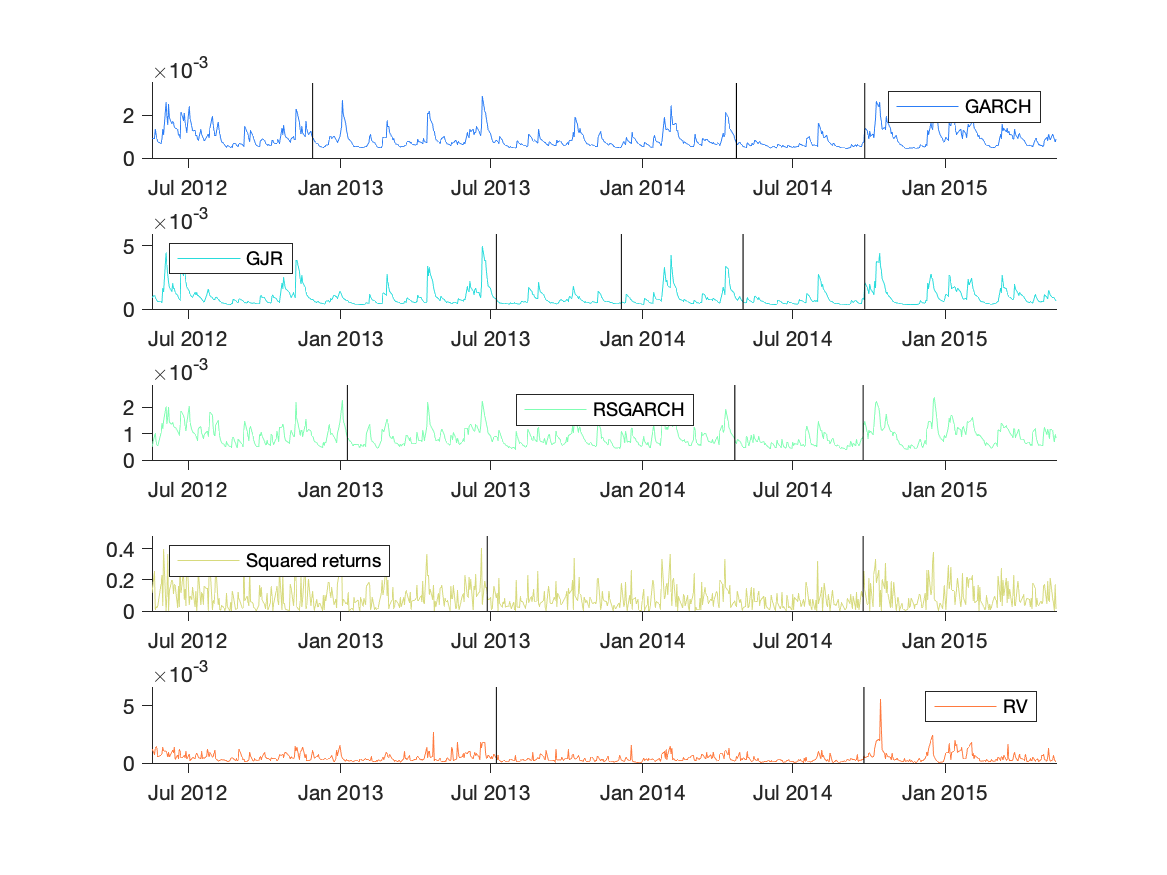
\includegraphics[width=1\textwidth]{Peimin/Volatility_SP_CP_GARCH_GJR_RSGARCH.png}
		\caption{
		Cluster Partition Volatility of S\&P 500 index.
			In Panel 1-3, we show conditional volatility estimated by {\color{blue} GARCH}, {\color{cyan}GJR-GARCH} and {\color{green}RSGARCH}. Panel 4-5 present {\color{yellow}squared returns} and {\color{red}realised volatility}. For each volatility series, we use cluster partition method to get different sequences.
			Codes can be found in \url{https://github.com/wzj5163/Cluster-partition-volatility/tree/main/Insample_estimation/Insample_estimation_20220905}.
		}
		\label{fig13_sp} %% label for entire figure
	\end{center}
\end{figure}

\begin{figure}[htbp]
	\begin{center}
		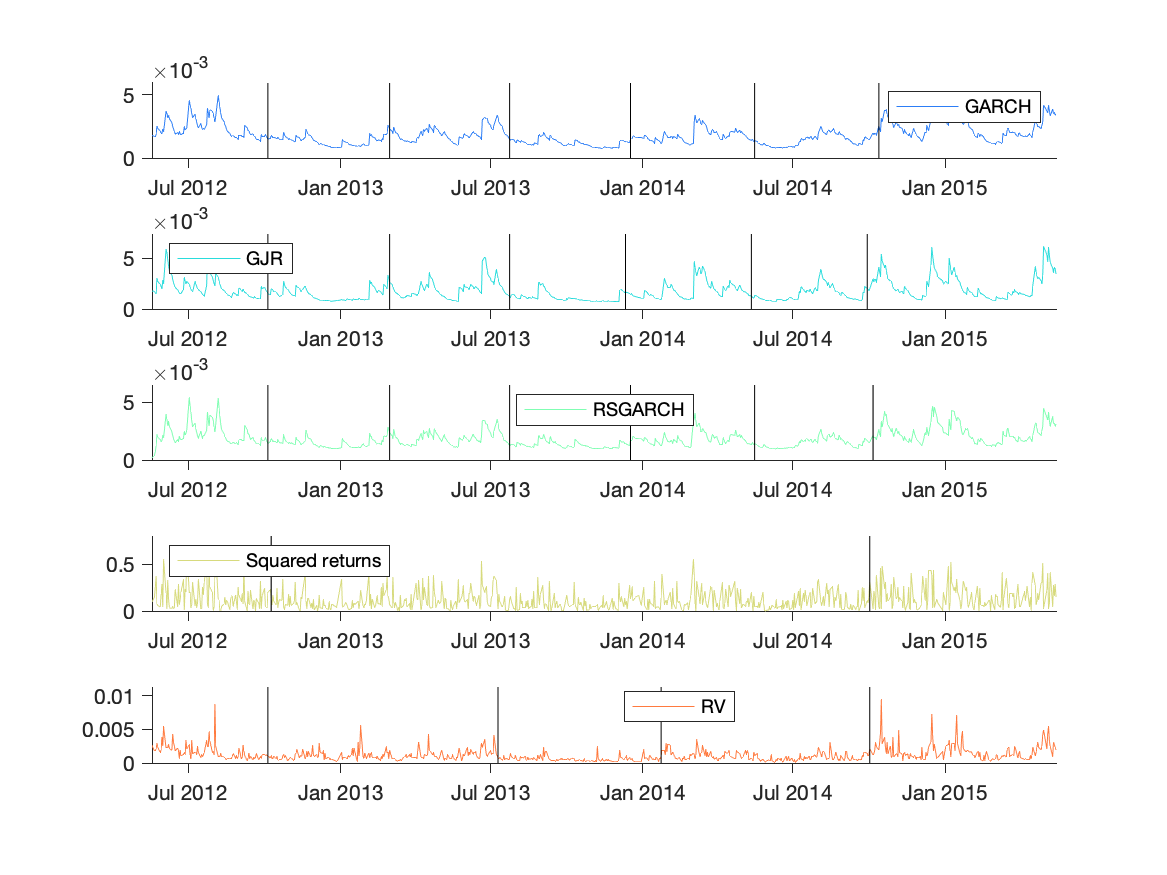
\includegraphics[width=1\textwidth]{Peimin/Volatility_DAX_CP_GARCH_GJR_RSGARCH.png}
		\caption{
		Cluster Partition Volatility of dx 30 index.
			In Panel 1-3, we show conditional volatility estimated by GARCH, GJR-GARCH and RSGARCH. Panel 4-5 present squared returns and realised volatility. For each volatility series, we use cluster partition method to get different sequences. Codes can be found in \url{https://github.com/wzj5163/Cluster-partition-volatility/tree/main/Insample_estimation/Insample_estimation_20220905}.
		}
		\label{fig13_dax} %% label for entire figure
	\end{center}
\end{figure}

\begin{figure}[htbp]
	\begin{center}
		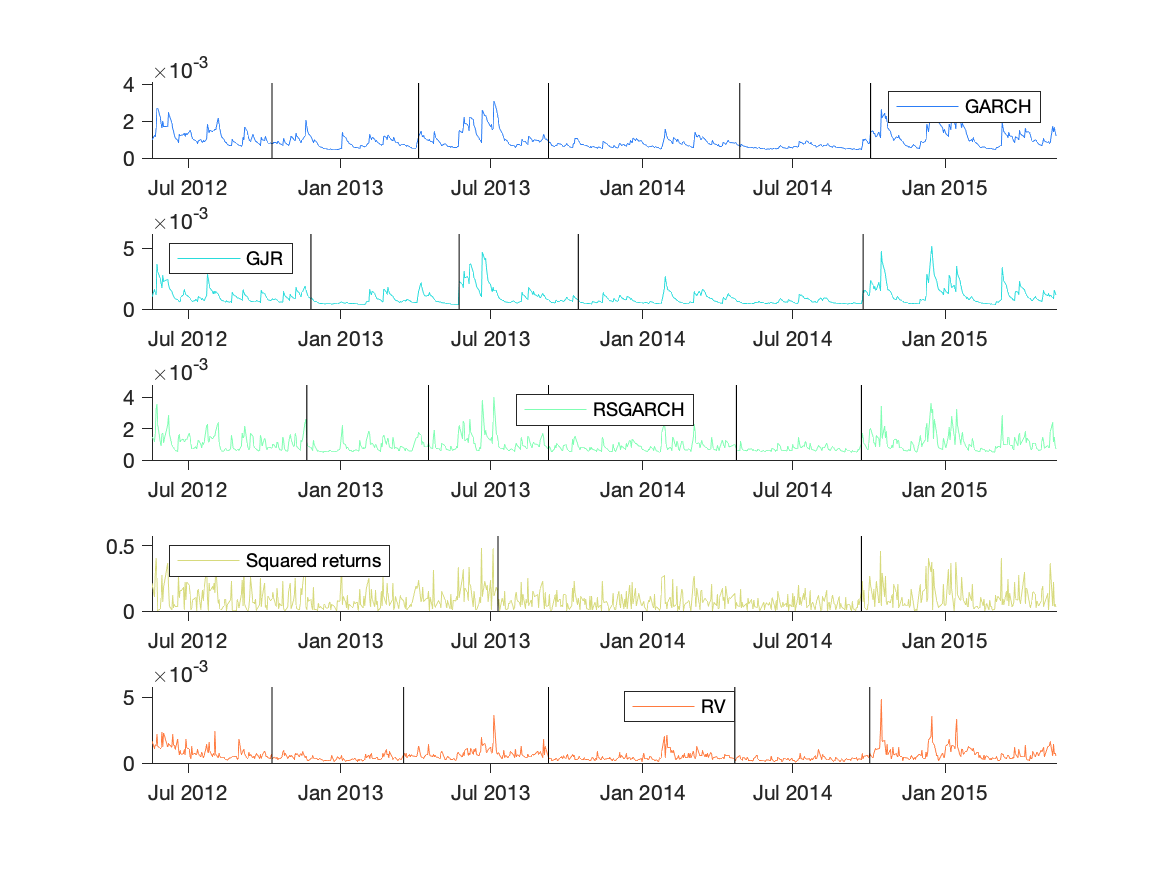
\includegraphics[width=1\textwidth]{Peimin/Volatility_FTSE_CP_GARCH_GJR_RSGARCH.png}
		\caption{
  Cluster Partition Volatility of FTSE 100 index.
			In Panel 1-3, we show conditional volatility estimated by GARCH, GJR-GARCH and RSGARCH. Panel 4-5 present squared returns and realised volatility. For each volatility series, we use cluster partition method to get different sequences.
			Codes can be found in \url{https://github.com/wzj5163/Cluster-partition-volatility/tree/main/Insample_estimation/Insample_estimation_20220905}.
		}
		\label{fig13_ftse} %% label for entire figure
	\end{center}
\end{figure}

\begin{figure}[htbp]
	\begin{center}
		\subfigure[S\&P 500 index]{
			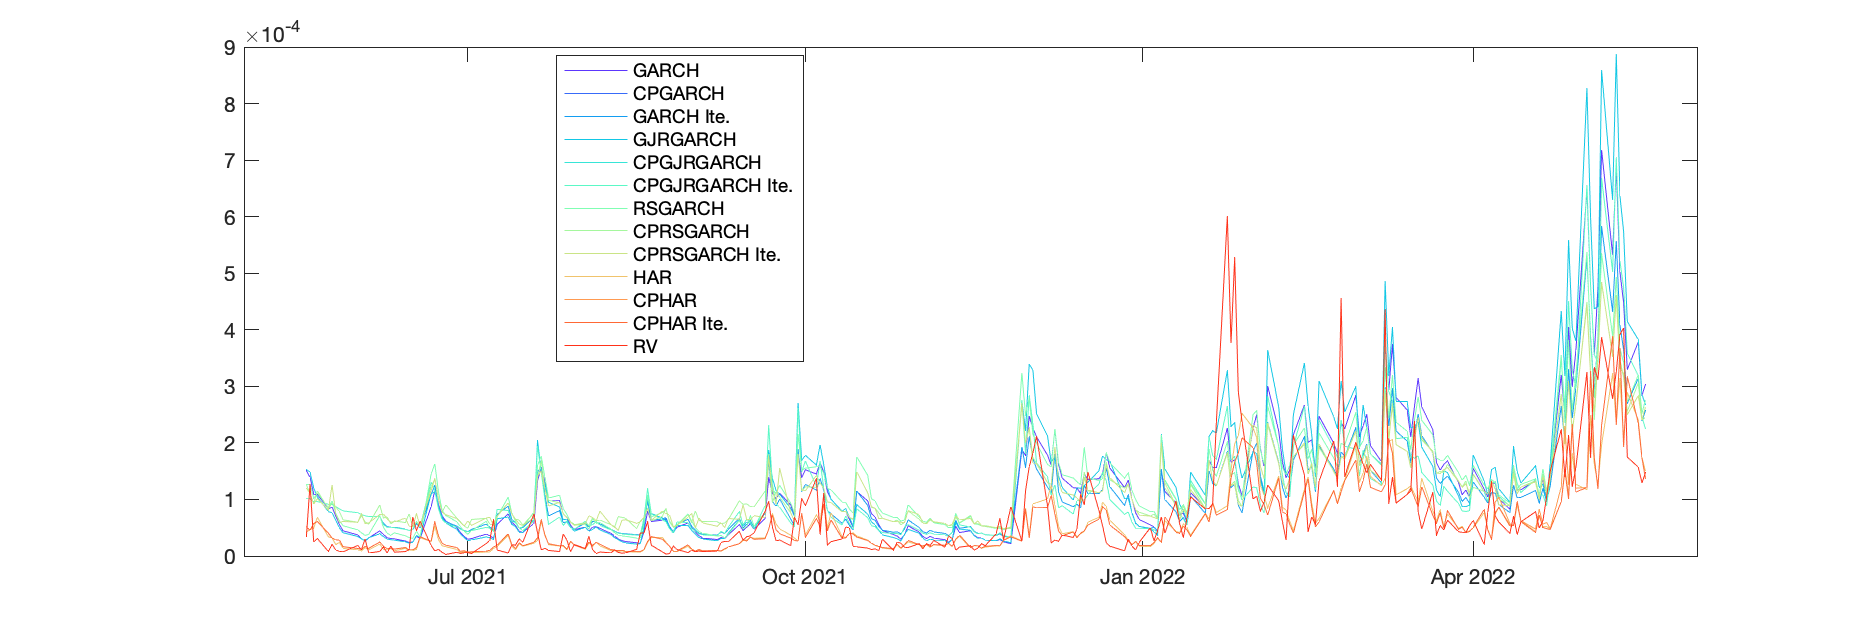
\includegraphics[width=0.8\textwidth]{Peimin/volatility_forecast_allmodel_SP.png}\label{fig16_sp}
		}
		\subfigure[DAX 30 index]{
			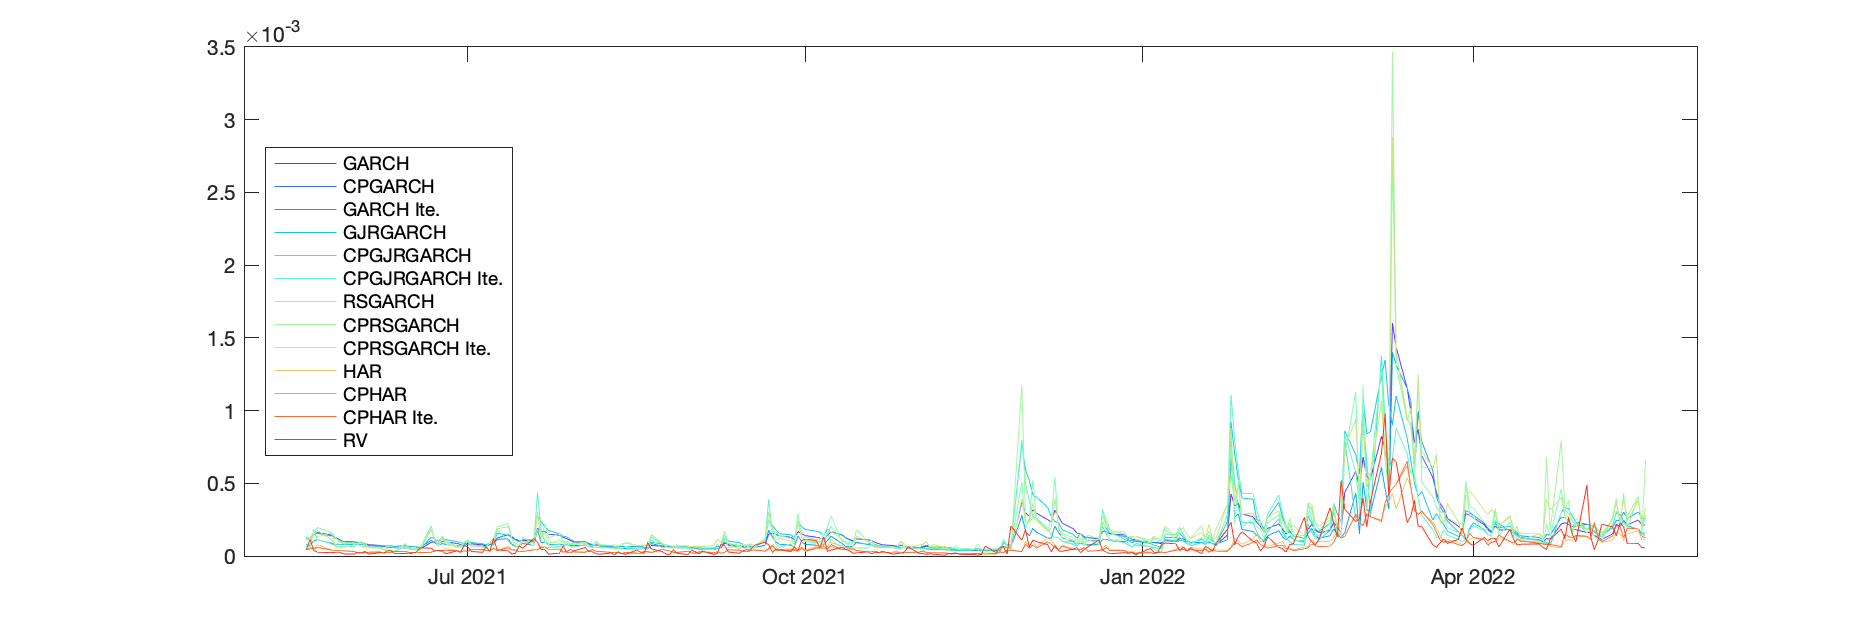
\includegraphics[width=0.8\textwidth]{Peimin/volatility_forecast_allmodel_DAX.png}\label{fig16_dax}
		}
		\subfigure[FTSE 100 index]{
			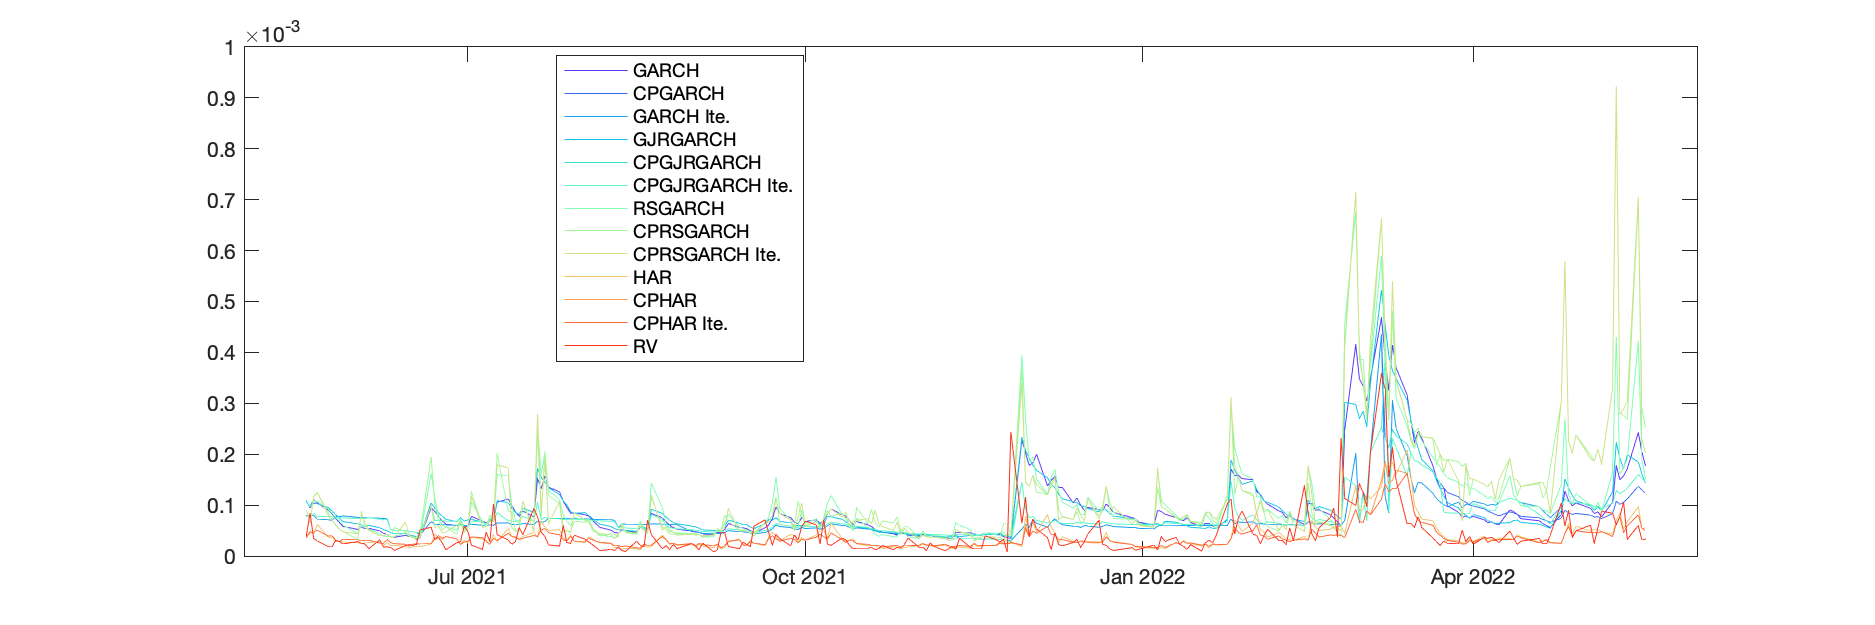
\includegraphics[width=0.8\textwidth]{Peimin/volatility_forecast_allmodel_FTSE.png}\label{fig16_ftse}
		}
		\caption{
		Volatility forecast}
		\label{fig16} %% label for entire figure
	\end{center}
\end{figure}

\begin{figure}[htbp]
\centering
\begin{minipage}[t]{0.48\textwidth}
\centering
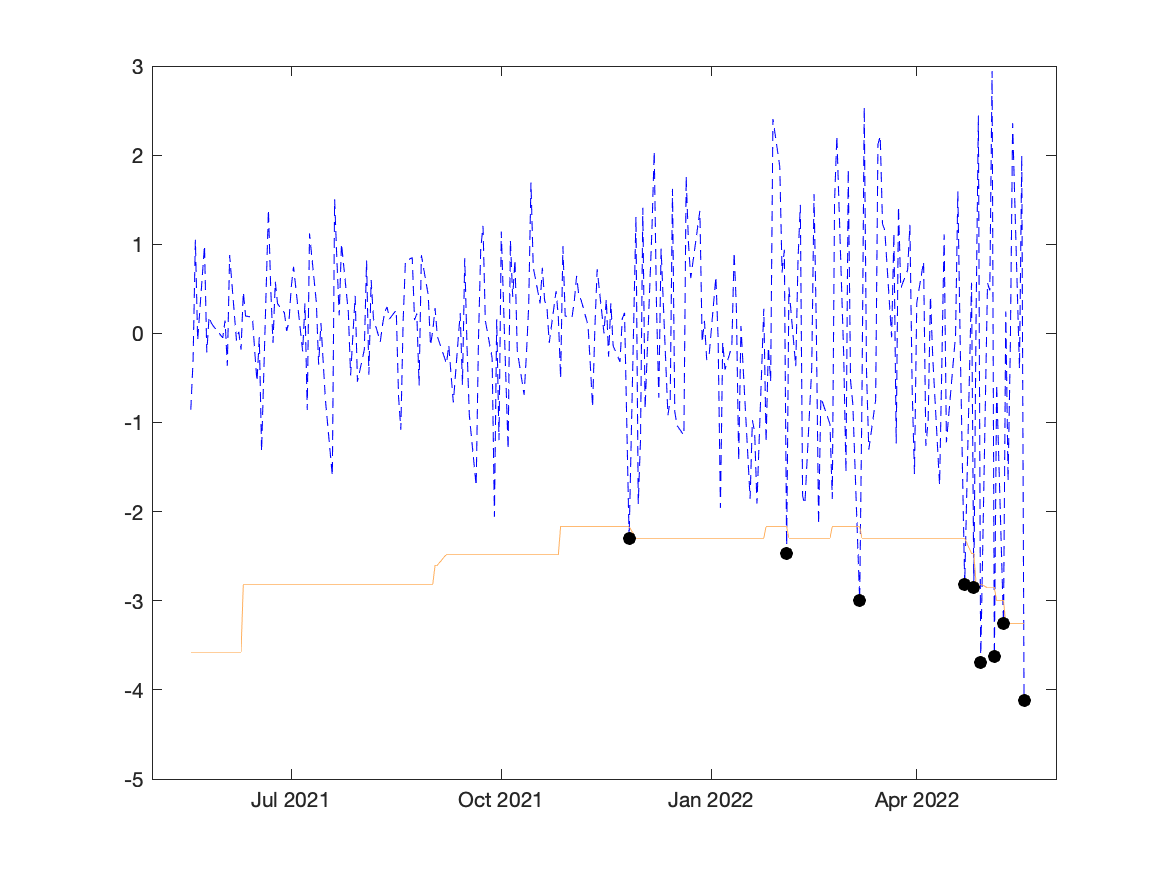
\includegraphics[width=6cm]{Peimin/VaR_HS_99.png}
\caption{Historical simulation}
\end{minipage}
\begin{minipage}[t]{0.48\textwidth}
\centering
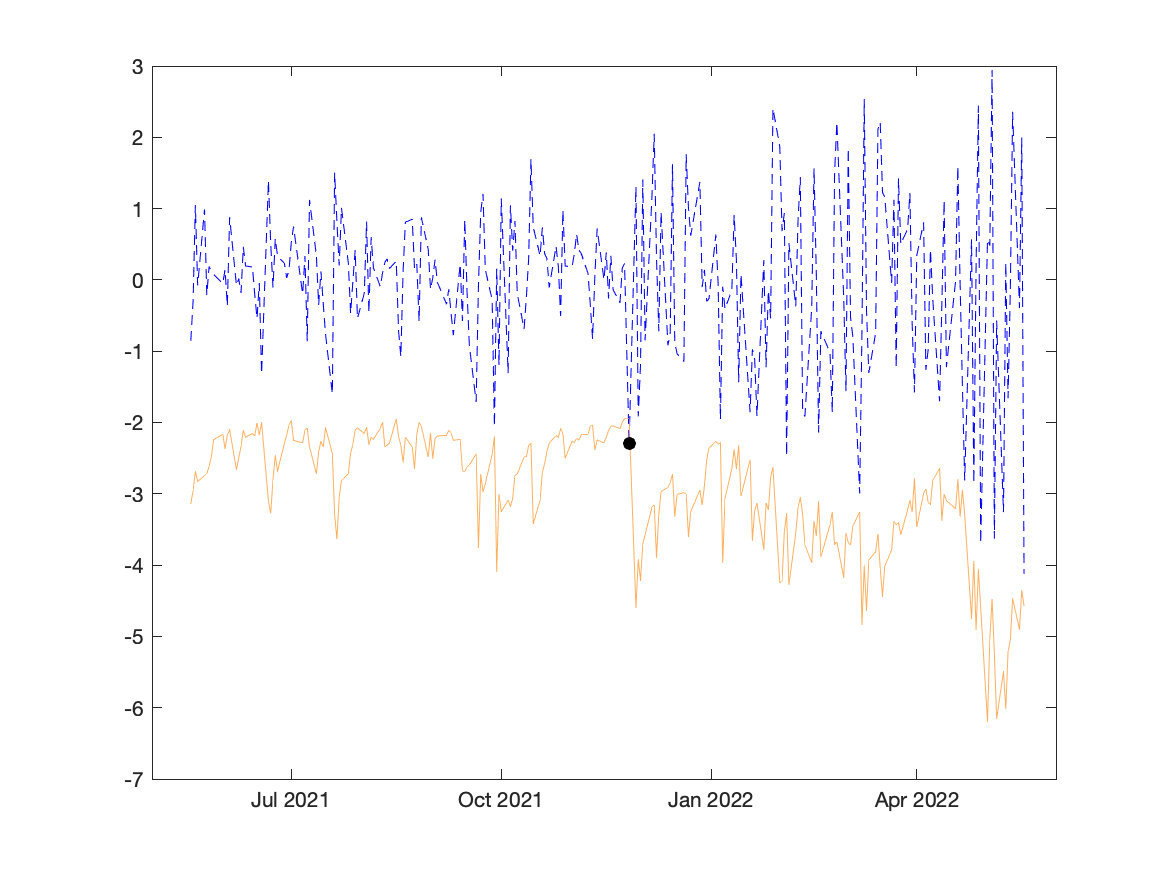
\includegraphics[width=6cm]{Peimin/VaR_CPRSGARCH_T_99.png}
\caption{CP-RSGARCH-t with $\alpha=0.01$}
\end{minipage}
\end{figure}

\label{EndOfDocument}
% \end{sloppypar}
\end{document}
